%%%%%%%%%%%%%%%%%%%%%%%%%%%%%%%%%%%%%%%%%%%%%%%%%%%%%%%%%%%%%%%%%%%%%%%%
%                                                                      %
%     File: Thesis_Implementation.tex                                  %
%     Tex Master: Thesis.tex                                           %
%                                                                      %
%     Author: Andre C. Marta                                           %
%     Last modified :  4 Mar 2024                                      %
%                                                                      %
%%%%%%%%%%%%%%%%%%%%%%%%%%%%%%%%%%%%%%%%%%%%%%%%%%%%%%%%%%%%%%%%%%%%%%%%

\chapter{Autorotation Mathematical Model}
\label{chapter:mathematical_model}


%%%%%%%%%%%%%%%%%%%%%%%%%%%%%%%%%%%%%%%%%%%%%%%%%%%%%%%%%%%%%%%%%%%%%%%%
\section{Vehicle Model}
\label{section:model}

When it comes to spacecraft vehicles, a very complex geometry is crucial to achieve a space mission. However, when one looks at different vehicles from old types like the Saturn V to new ones like the Falcon 9, the geometry is similar for the entire vehicle when it is launched. A giant launcher is used to put into orbit a smaller payload. This geometry is still in use and does not show a greater margin in progress in the following years, once one can understand from figure \ref{fig:rocket_models}, where three different vehicles are presented from different companies.

\begin{figure}[!htb]
    \centering
    \subfloat[Ariane 6 \cite{noauthor_european_nodate}\label{fig:ariane_6}]{
        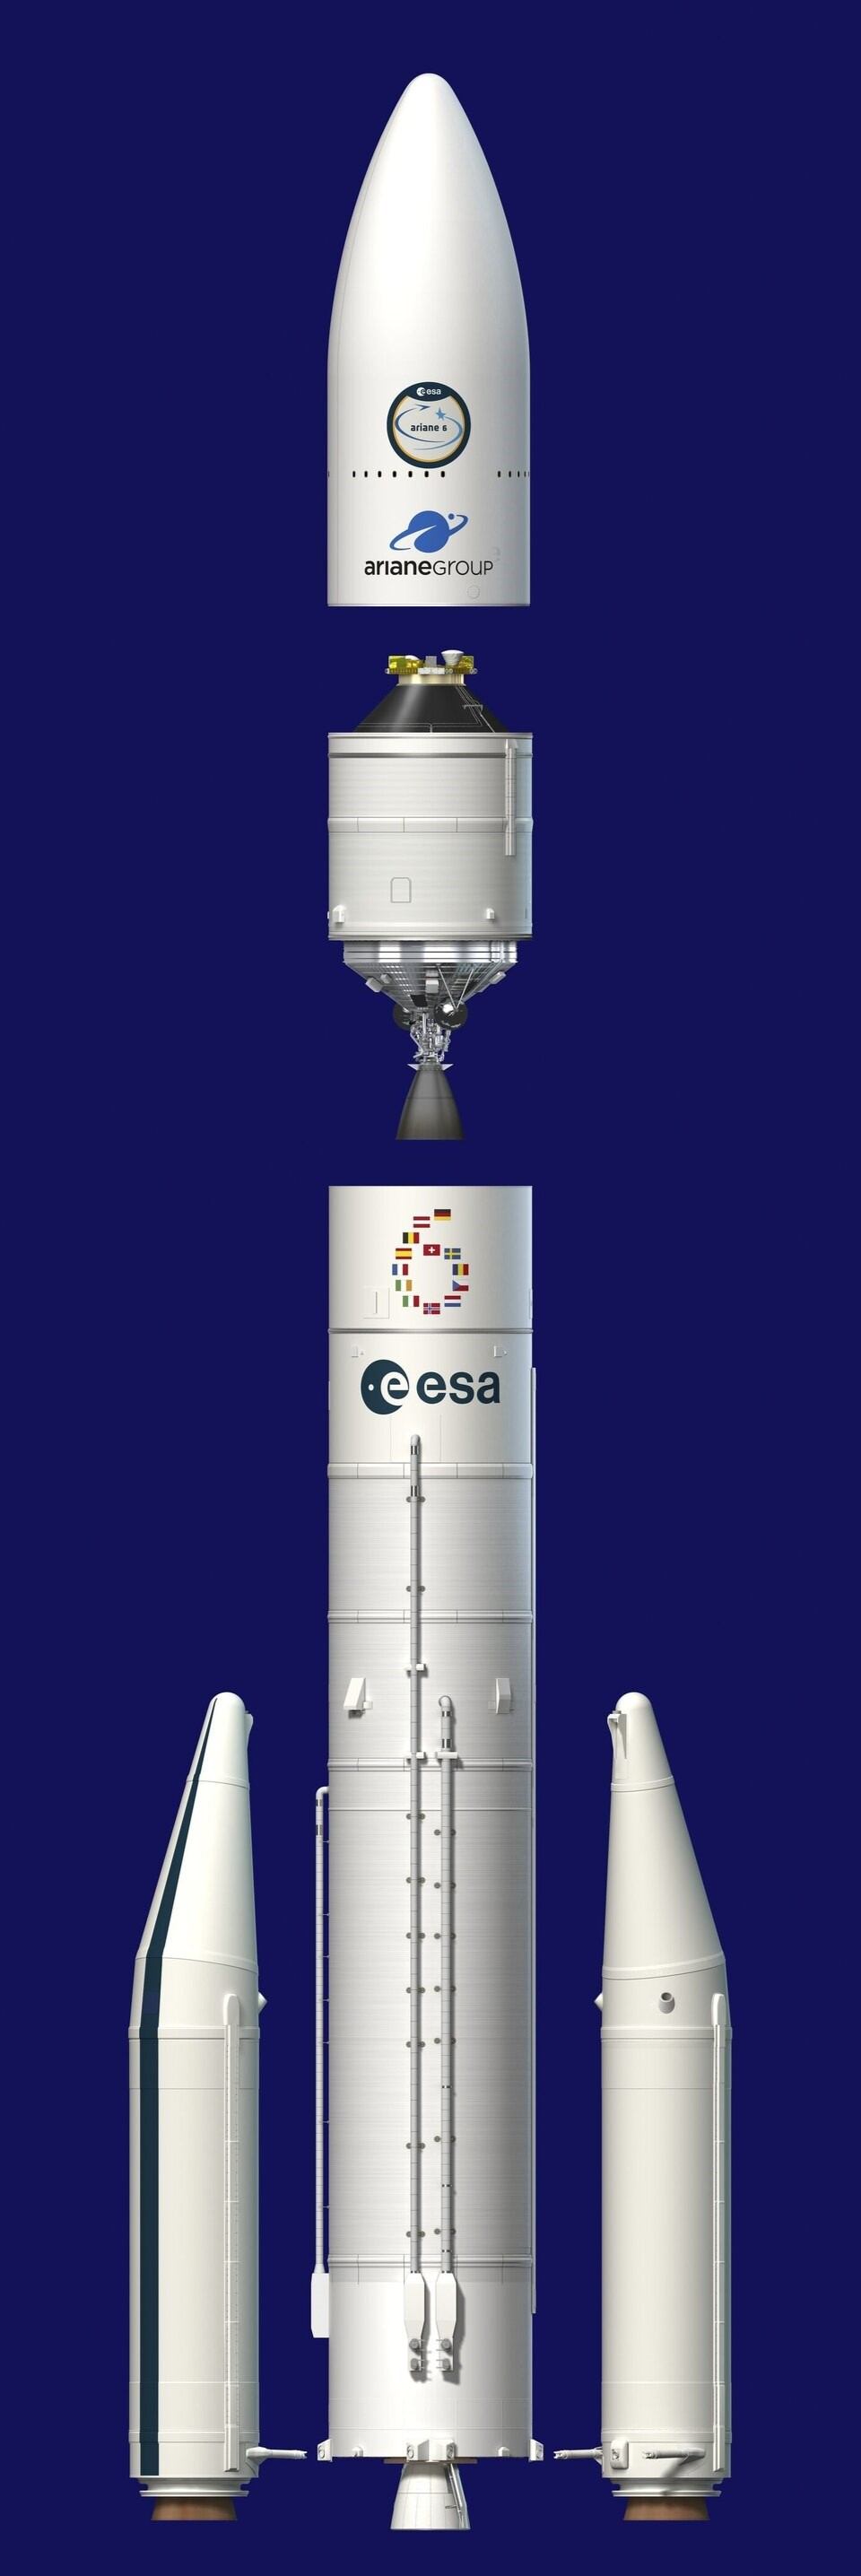
\includegraphics[height=7cm]{Figures/implementation/model/ariane_6.jpg}
    }\hfill
    \subfloat[Falcon 9 \cite{noauthor_spacex_nodate}\label{fig:falcon_9}]{
        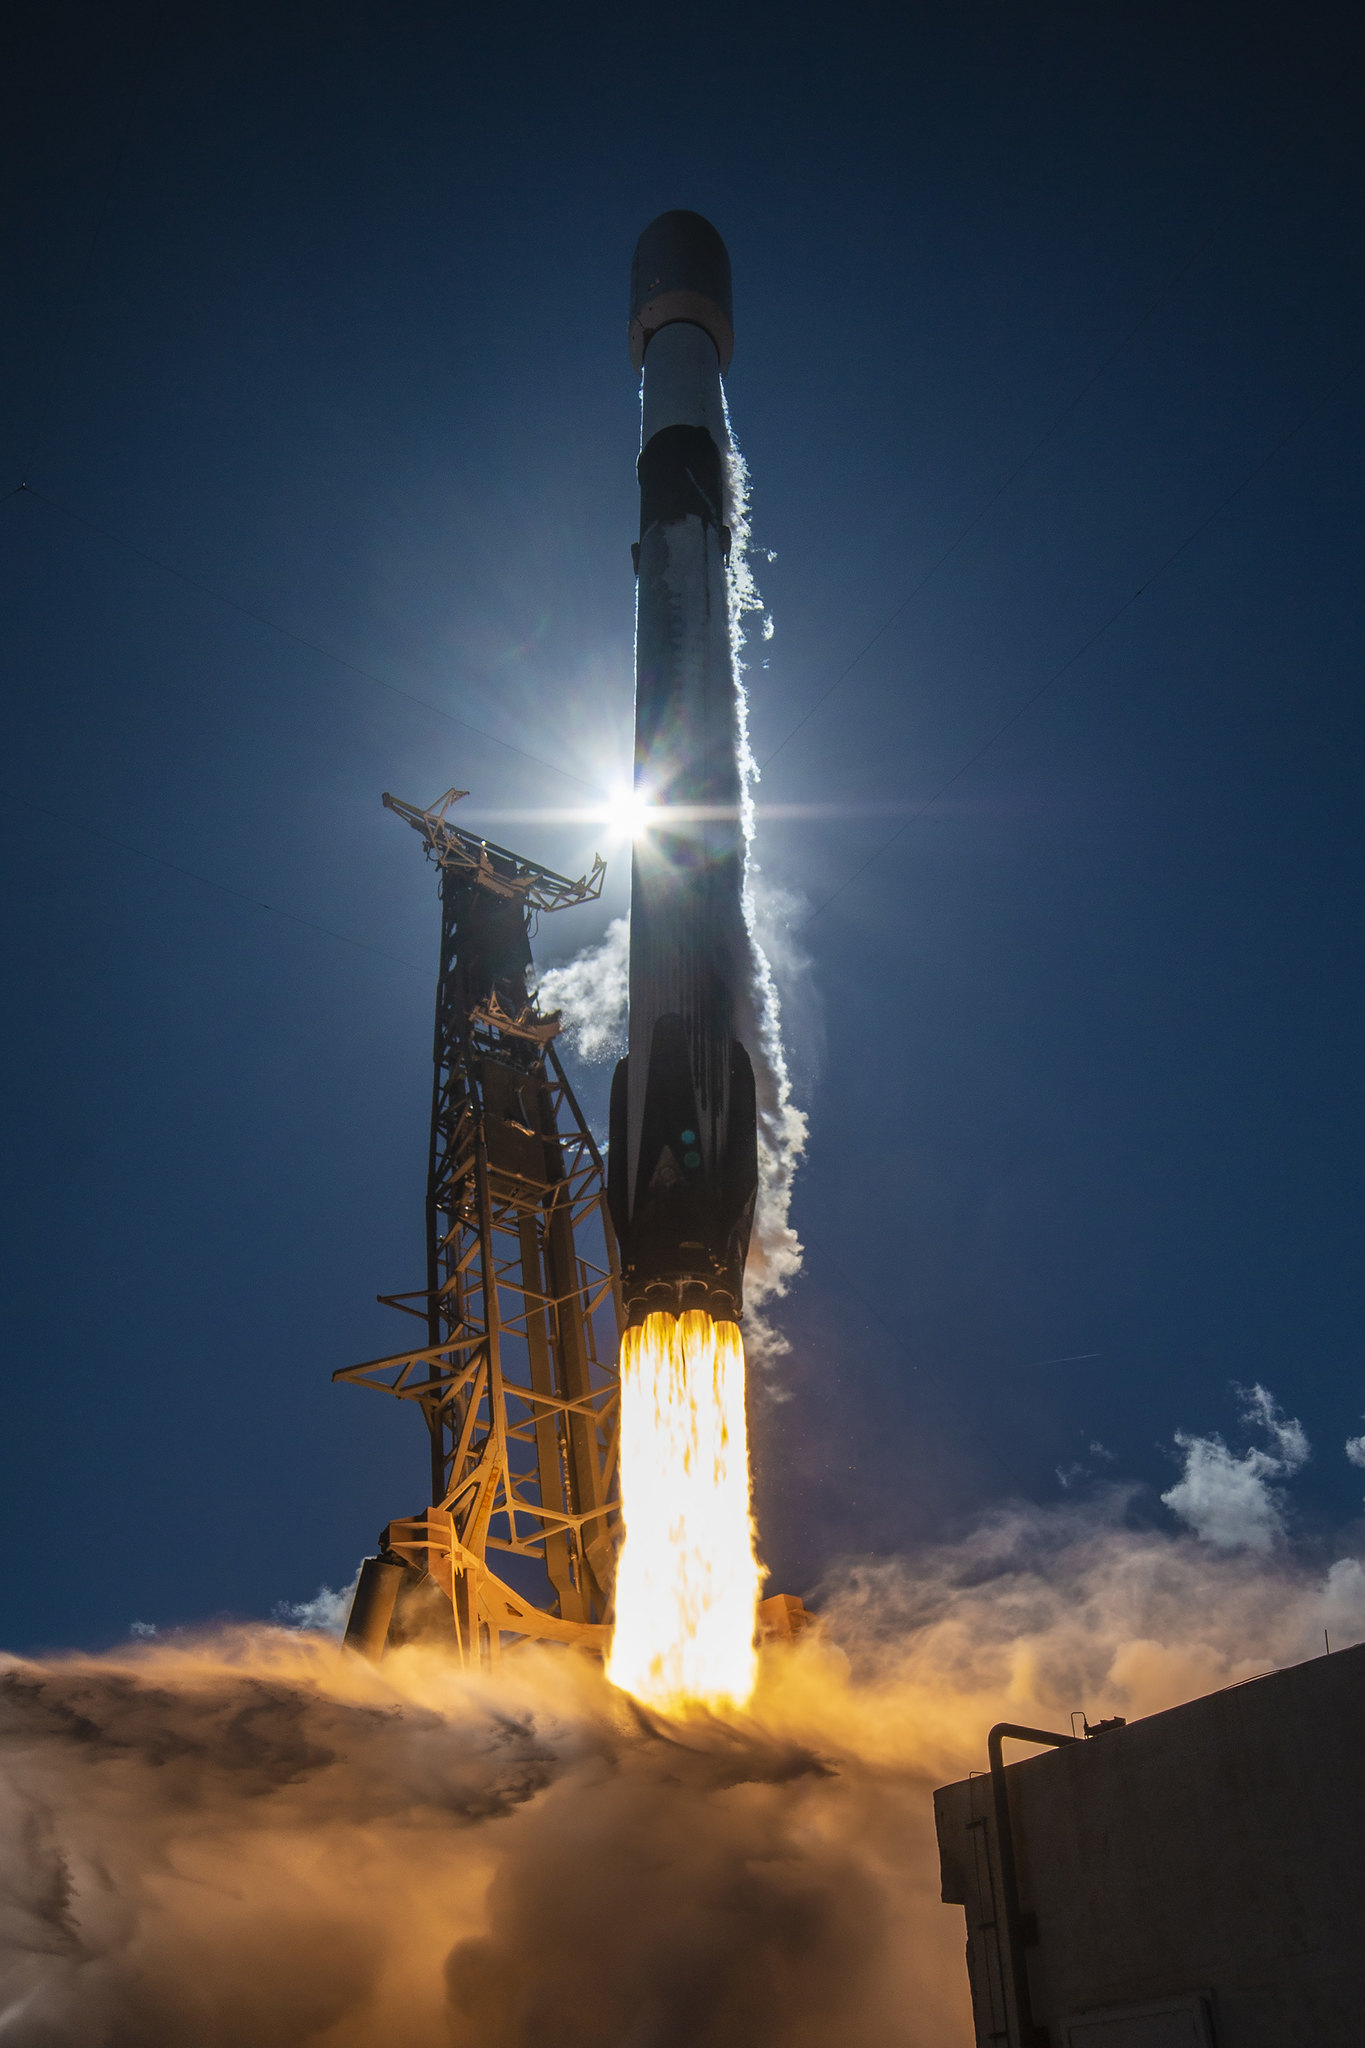
\includegraphics[height=7cm]{Figures/implementation/model/falcon_9.jpg}
    }\hfill
    \subfloat[New Shepard \cite{noauthor_blueorigin_nodate}\label{fig:new_shepard}]{
        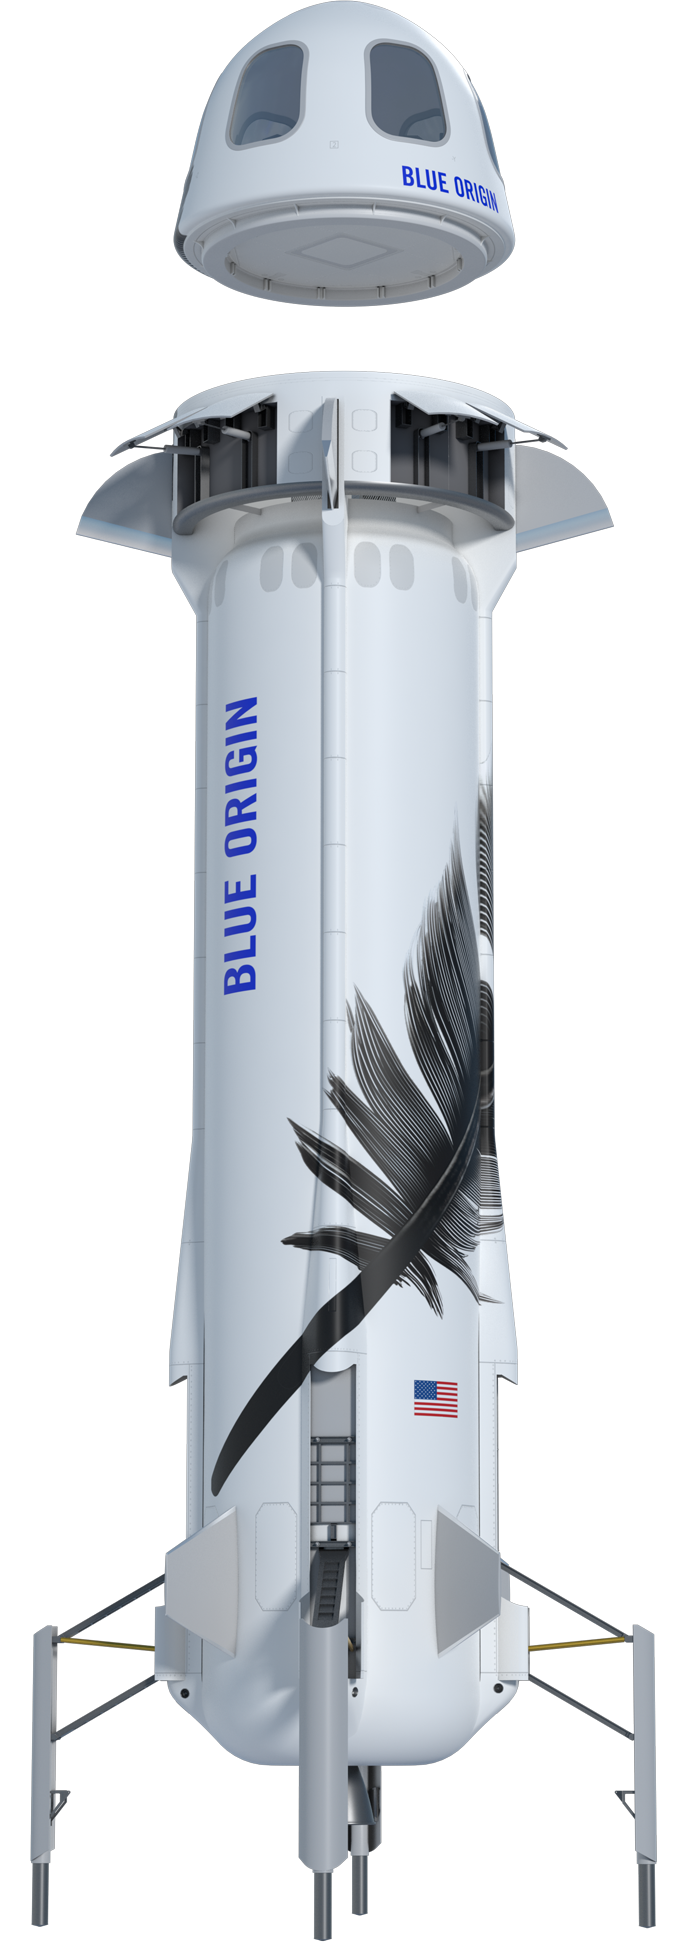
\includegraphics[height=7cm]{Figures/implementation/model/newshepard.png}
    }
    \caption{Spacecraft Vehicles operating nowadays}
    \label{fig:rocket_models}
\end{figure}

It is possible to understand that heavy launchers are mainly constructed under the same geometry: a cylinder. Also the previously referenced works \cite{maurer_project_nodate} and \cite{riegler_daedalus_2018} show a cylinder geometry for launchers Although it is a lighter and simpler vehicle which do not aim to achieve Earth's orbit. This means that the space industry still lies in cylinder format for its key component: the launcher.

So, before any other assumption, this thesis focus type of vehicle will be a simple cylinder with a rotor with a rotor on its top. Figure \ref{fig:vehicle_model}, presents the simplified vehicle considered. To easily define the geometry, it will be considered the geometry propreties shown in figure \ref{fig:vehicle_geometry}.


\begin{figure}[!htb]
    \centering
    \subfloat[Vehicle Model\label{fig:vehicle_model}]{
        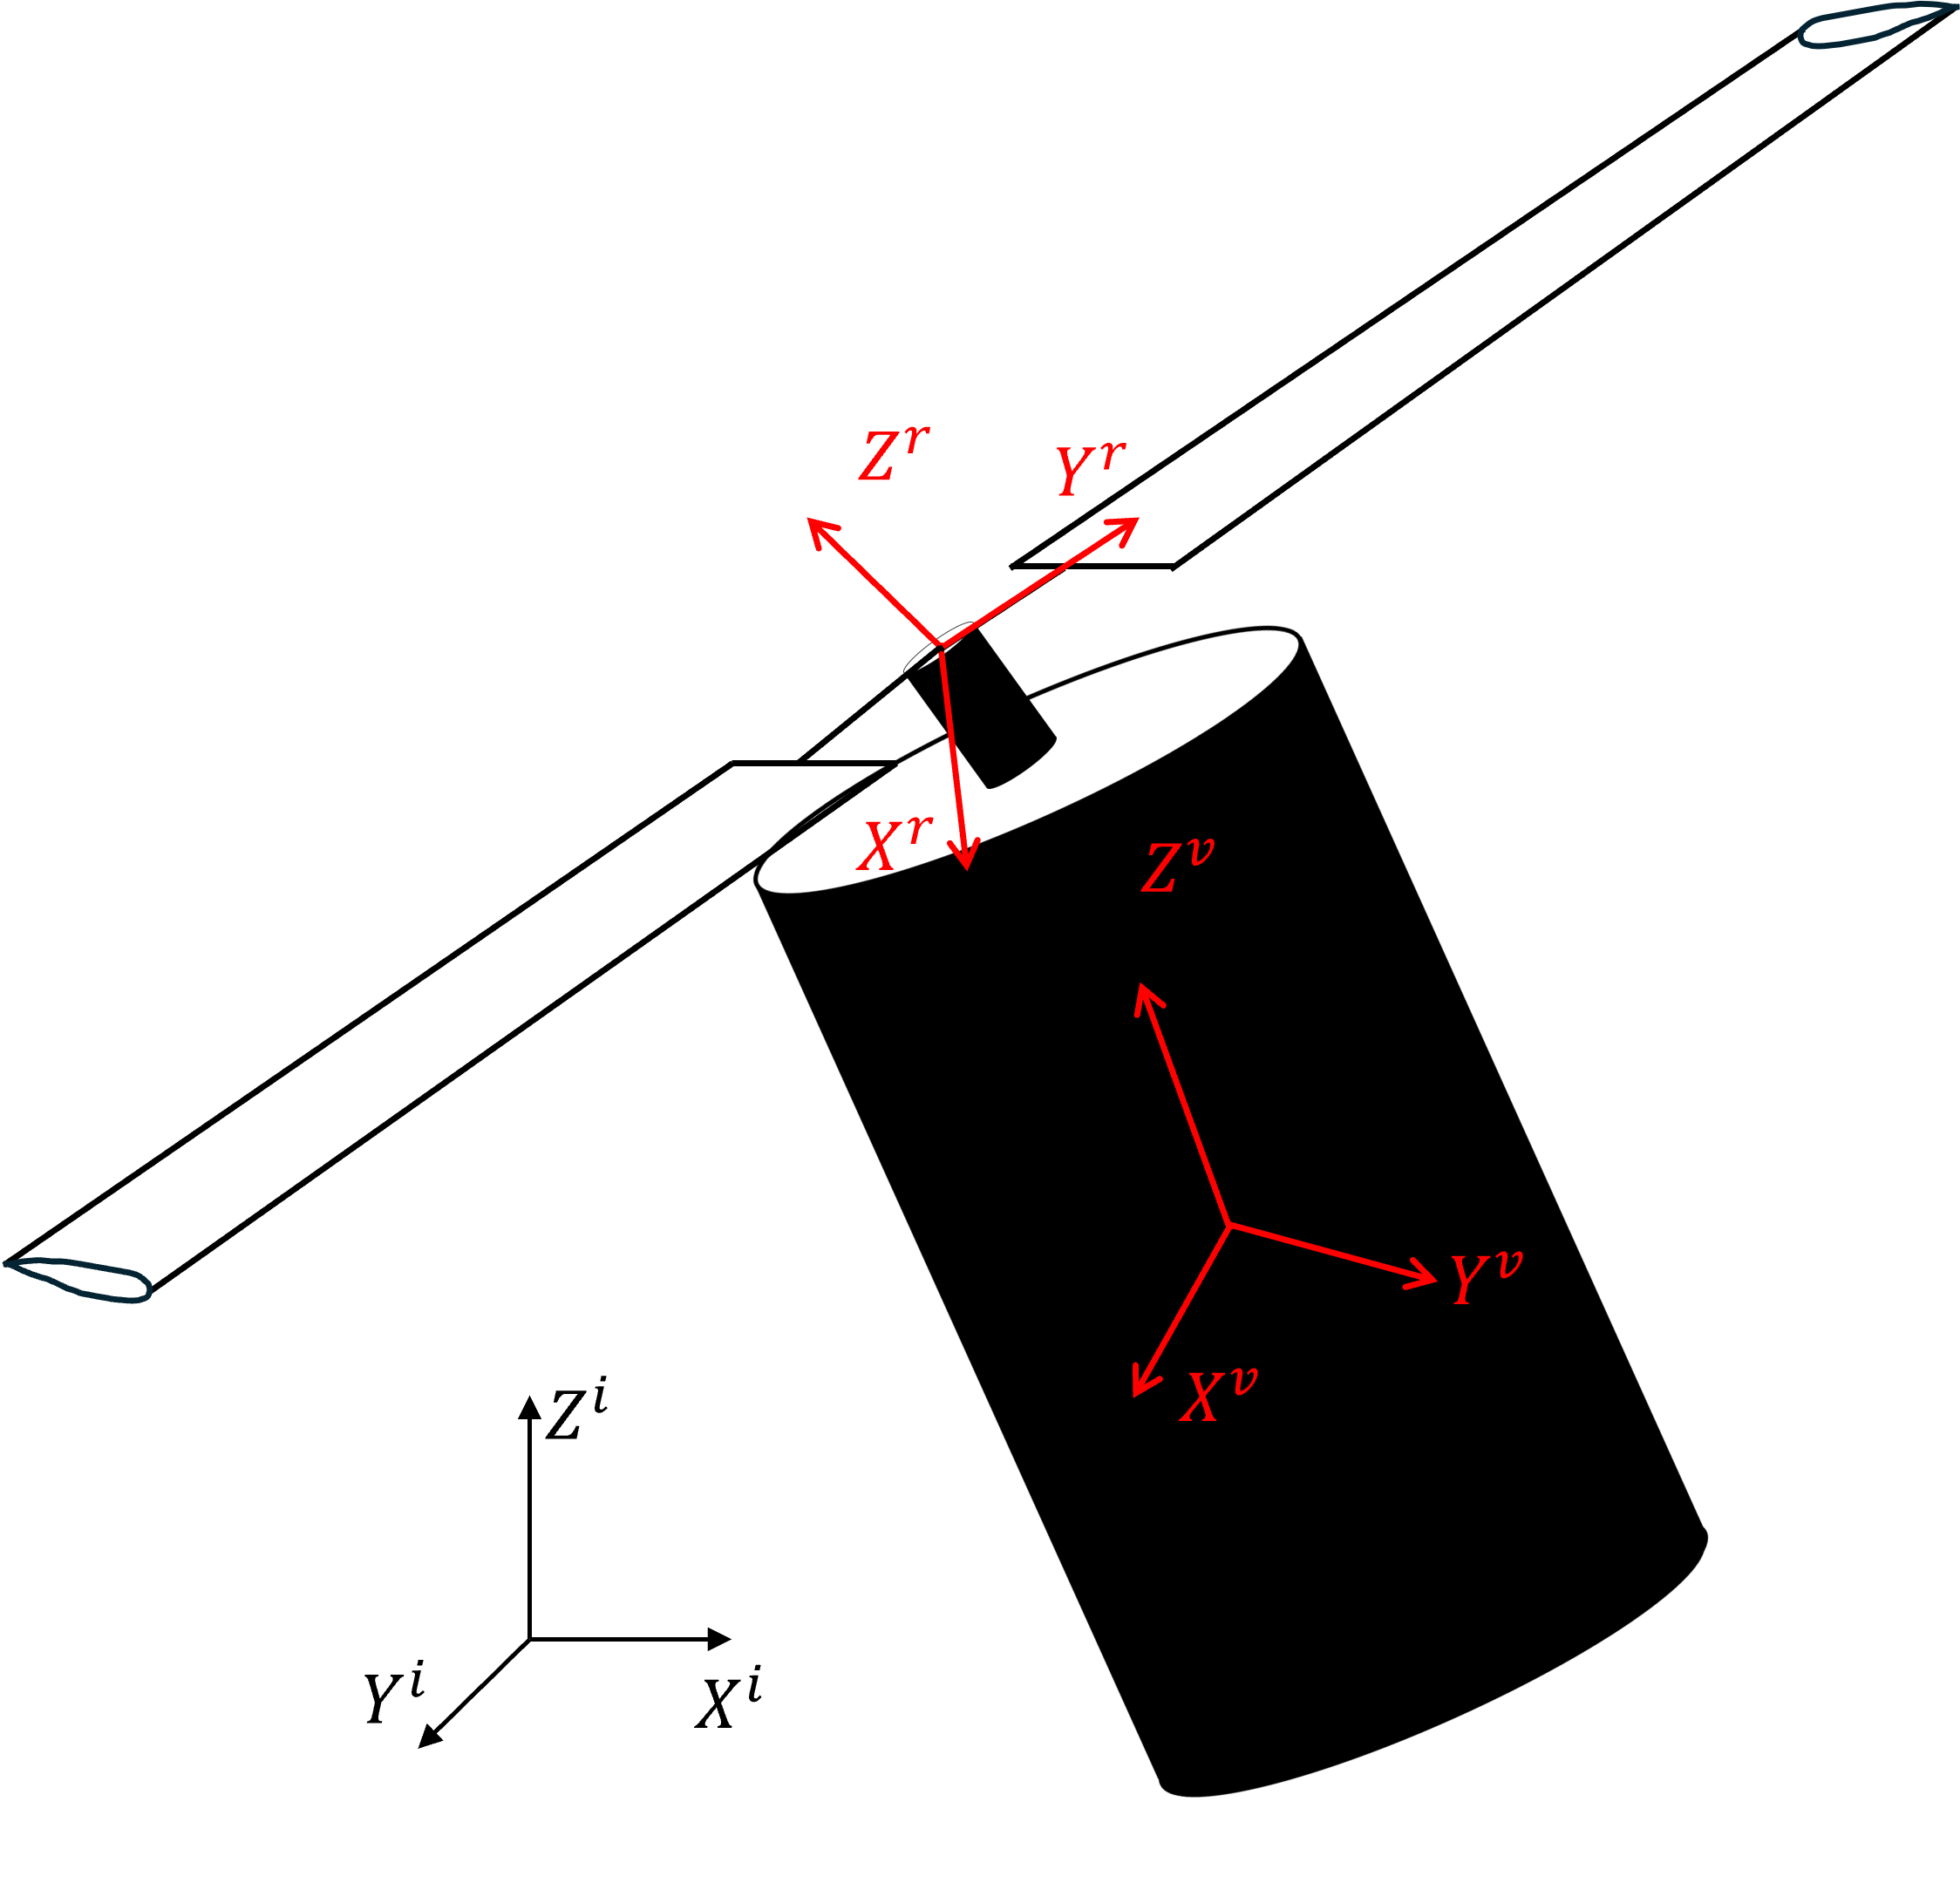
\includegraphics[height=6cm]{Figures/implementation/model/vehicle.png}
    }\hfill
    \subfloat[Vehicle Geometry proprieties\label{fig:vehicle_geometry}]{
        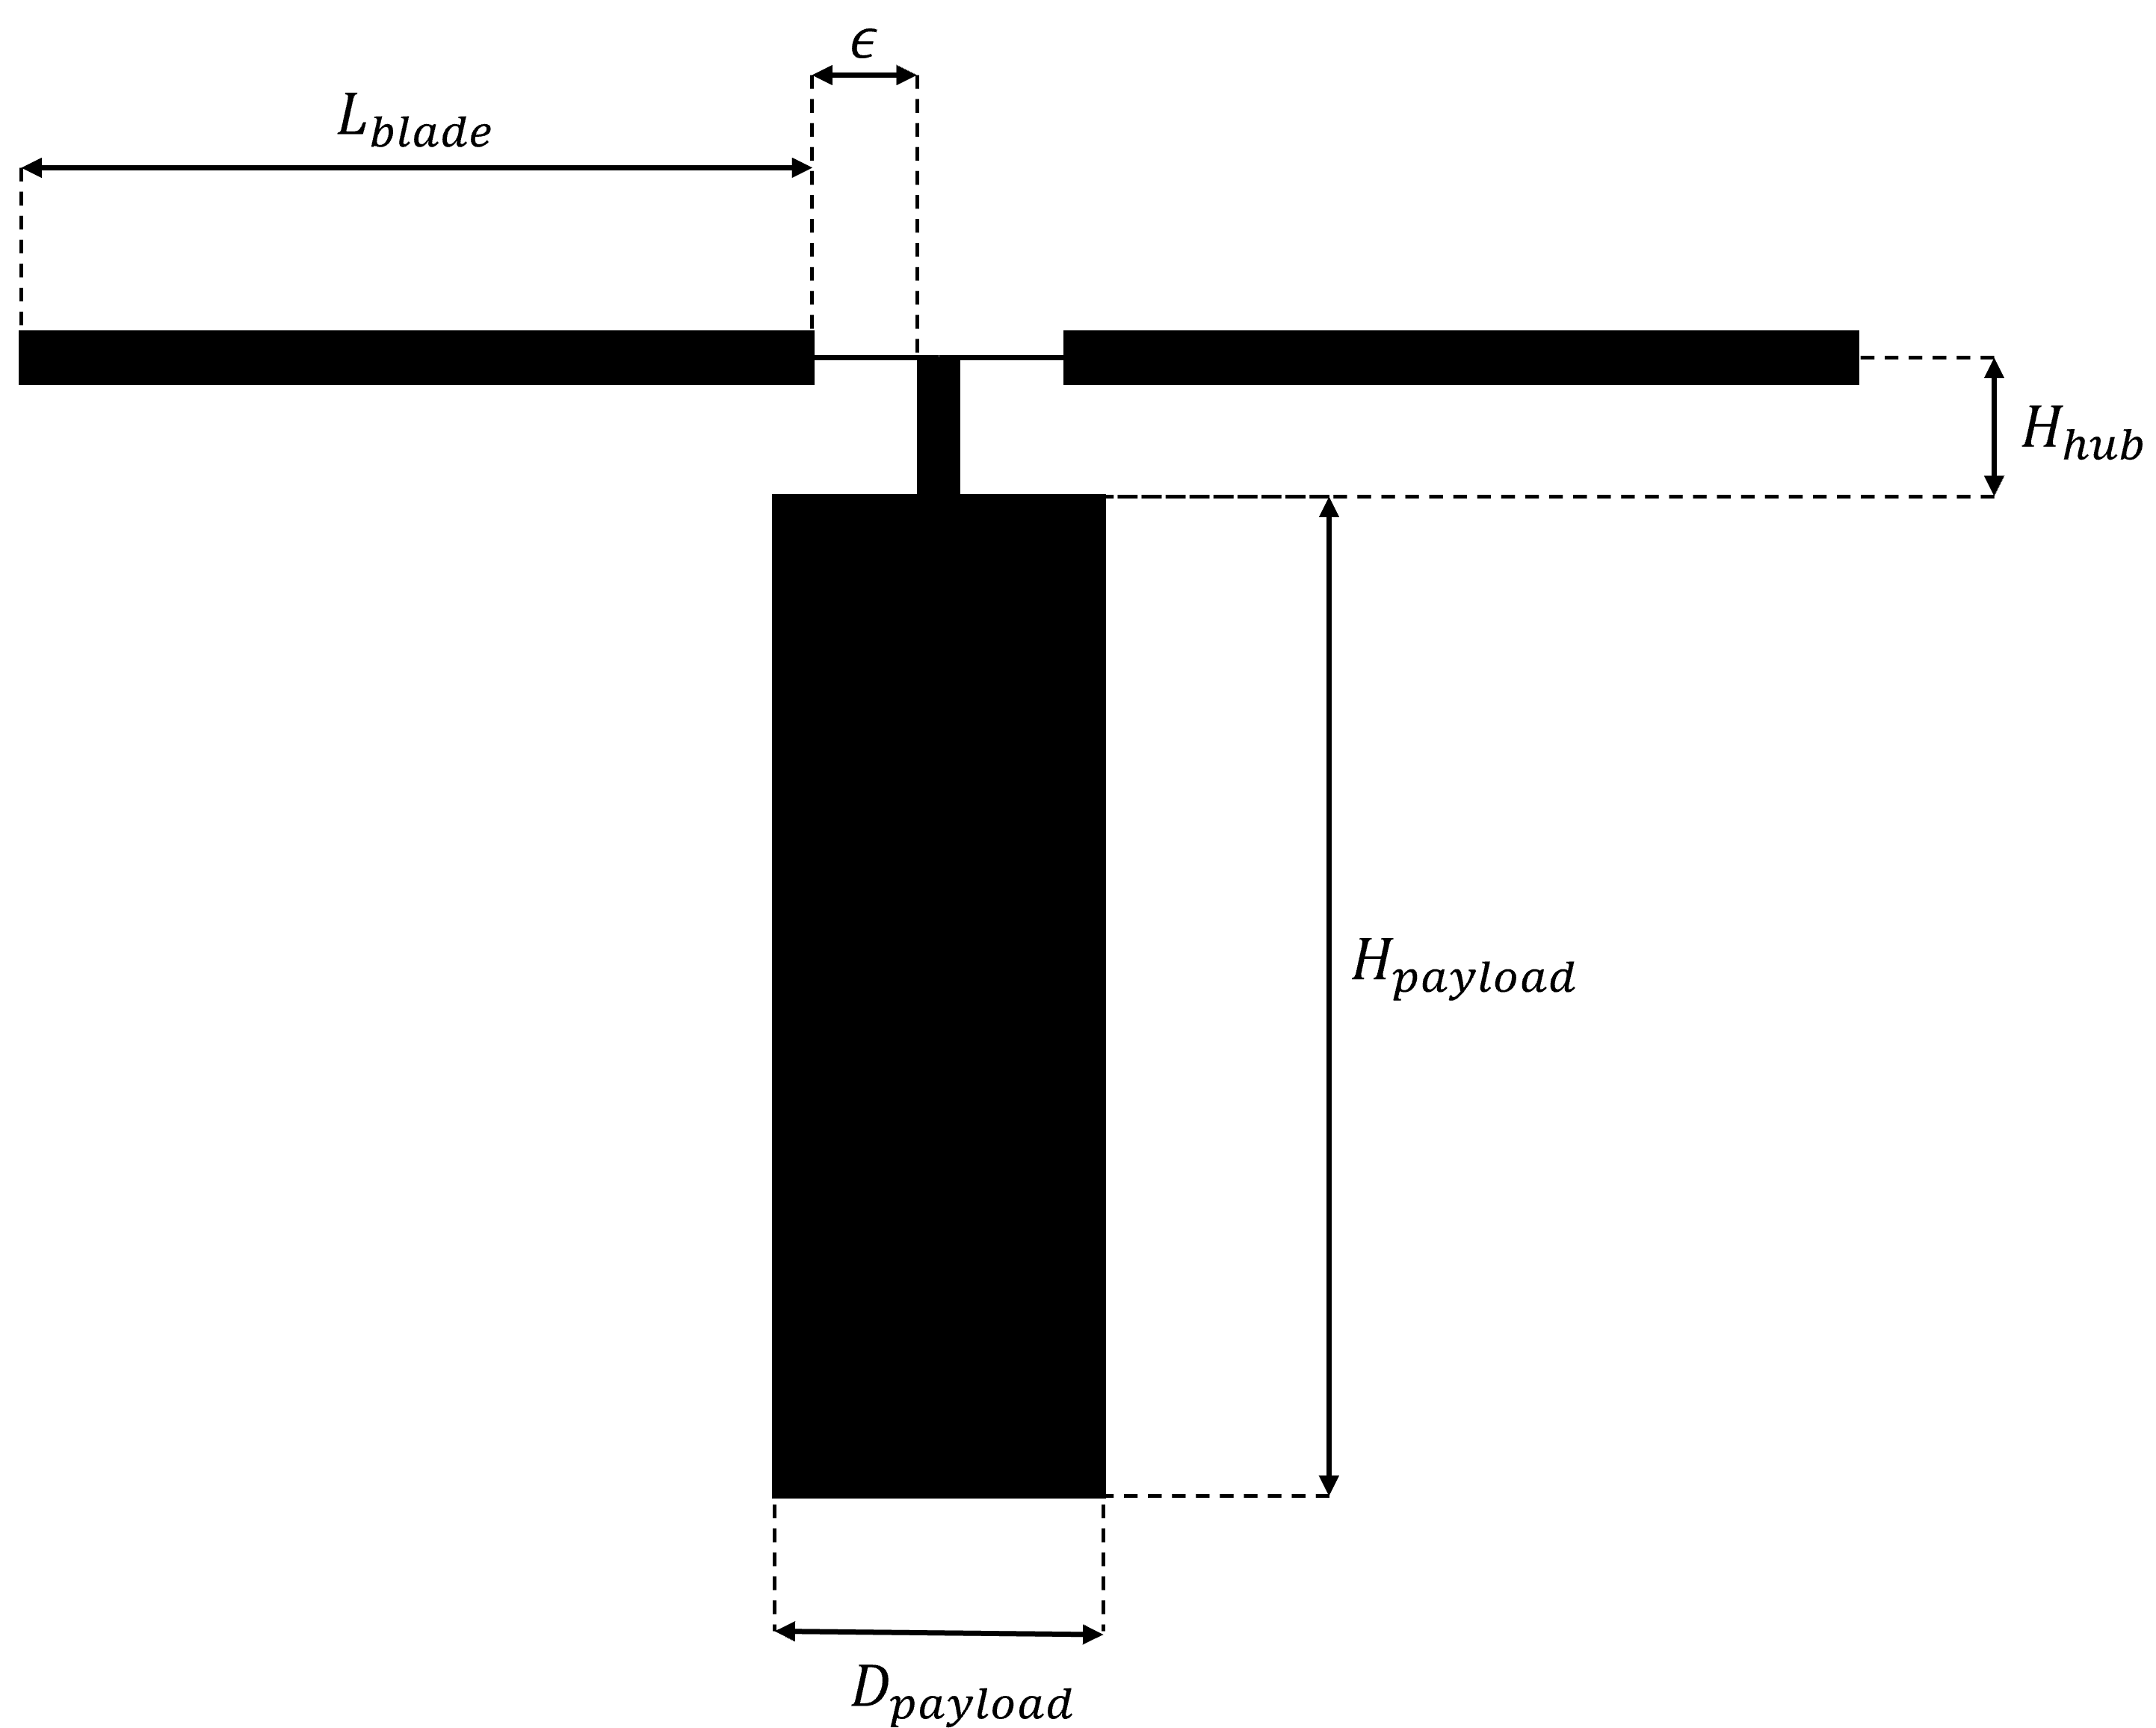
\includegraphics[height=6cm]{Figures/implementation/model/geometry_proprieties.png}
    }
    \caption{Vehicle}
    \label{fig:vehicle}
\end{figure}


\subsection{Model simplications and assumptions}
\label{section:model_assumptions}

\textcolor{blue}{meter as simplicações aqui}

\begin{itemize}
    \item o corpo é rígido
    \item tem movimento de translação e rotação nos 3 eixos
    \item é deprezada a rotação da terra
    \item a terra é plana
\end{itemize}

\textcolor{blue}{falar sobre as metologias de alguns livros para mostrar o que usar em cada uma das partes do projeto}

\subsection{Reference Frames}
\label{section:referece_frames}

For the development of the mathematical model that follows and considering what was present in previous section \ref{section:model_assumptions} one must start by considering the reference frames which define the vehicle's dynamics. On figure \ref{fig:vehicle_model} the three principal references are presented: Earth referece frame, $O^i$, vehicle referece frame $O^v$ and rotor frame $O^r$.

The Earth frame, $O^i$, is a inertial frame positioned in any point of the Earth surface. It is also called \textit{Navigation Frame} once it rotates with Earth and it is very handy when planes to travel from one point to another \cite{soler_fundamentals_2014}. On other hand, the vehicle frame, $O^v$,  or body frame \cite{soler_fundamentals_2014} is a system axes centered in any point of the symmetry plane of the aircraft. In this case, the $O^v$ is position at the \gls{cg} of the vehive considering a two point mass system, one for the payload and one for the recovery system. The $O^v$ as its $z^v$-axis aligned from the \gls{cg} as shwon in figure \ref{fig:vehicle_model} for orietation reference. Finally, the rotor axes system, $O^r$ is centered in the rotor's hub and is aligned and has the same orietation as the $O^v$ reference frame.


\begin{figure}[!htb]
    \centering
        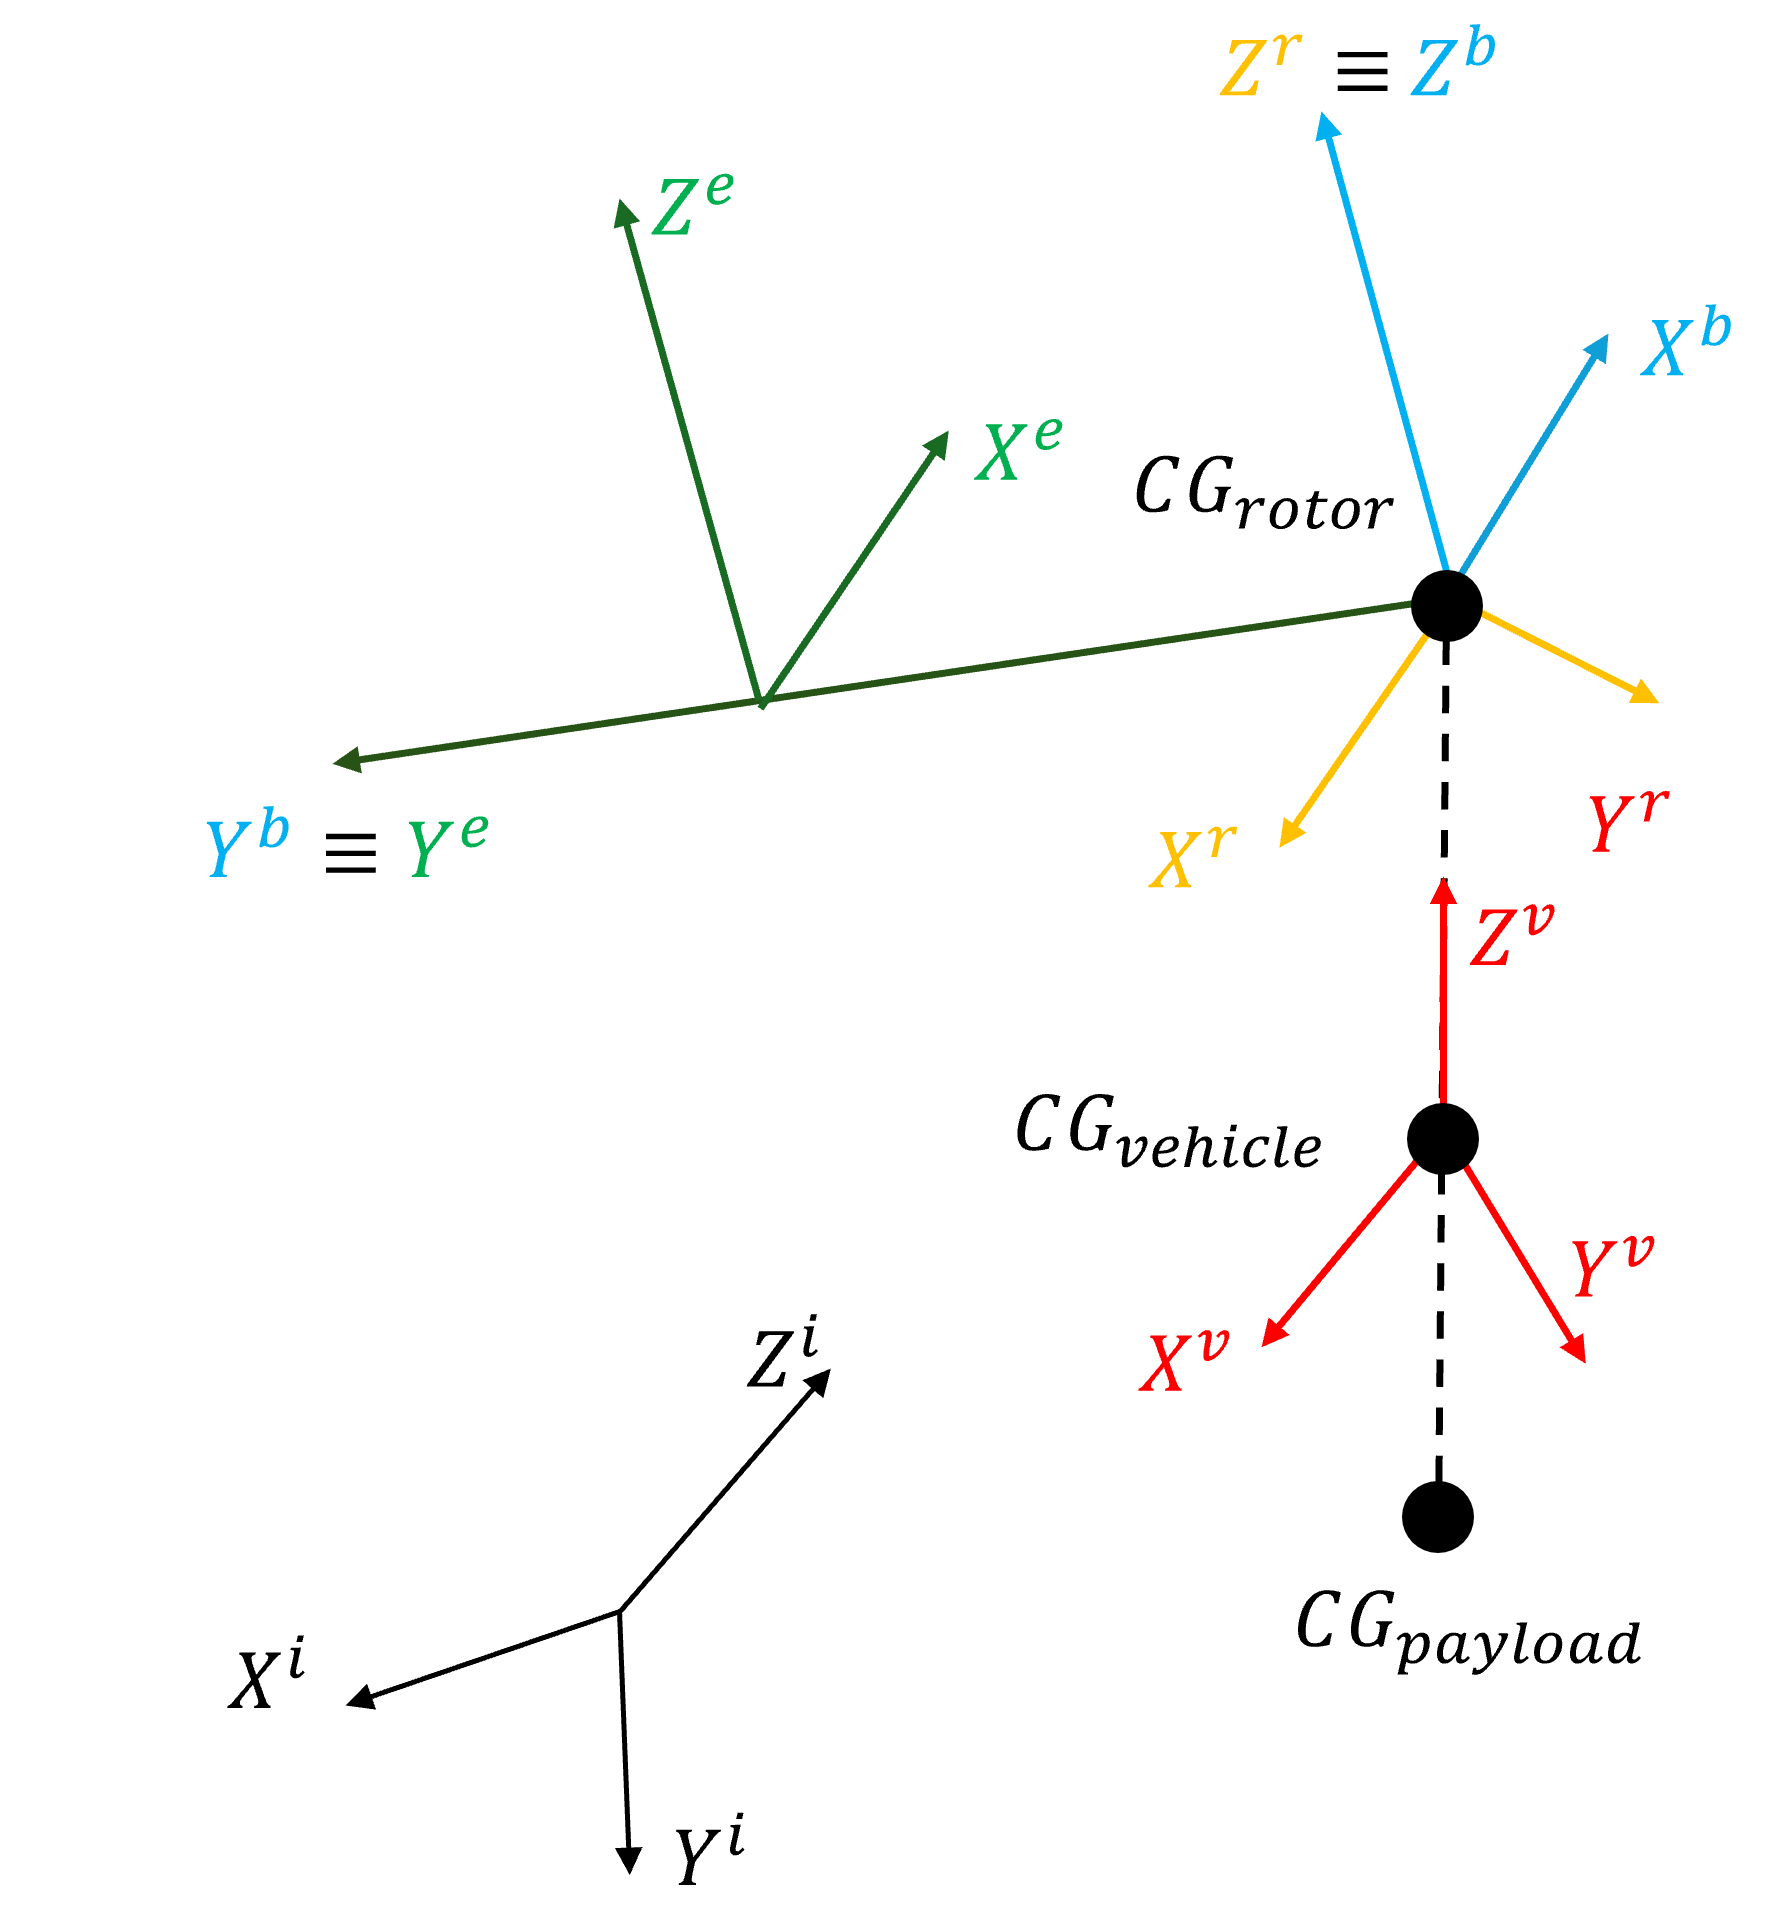
\includegraphics[width=8cm]{Figures/implementation/model/reference_frames_img.png}
        \caption{Model reference frames relation - as a simplication the figure was designed considering the that the viewer is aligned with $O^v \equiv O_r$ and the $O_i$ is rotated}
        \label{fig:reference_frames_img}
\end{figure}

The vehicle frame is positioned at the \gls{cg} of the vehicle total system and can be write in the $O^i$ as navigation coordinates,

\begin{equation}
    \mathbf{p}^i_{CG_{vehicle}} = \begin{bmatrix} x & y & z \end{bmatrix}^T \in \mathbb{R}^3.
\end{equation}

However, for moments calculations the position of the vehicle total system's \gls{cg} is a crucial point. As a simplification, previous mentioned in section \ref{section:model_assumptions}, the vehicle's \gls{cg} does not vary inside the vehicle. So, to determine the position of rotor's and payload's \gls{cg}, as presented in figure \ref{fig:reference_frames_img} relative to the overall system's \gls{cg} the vehicle´s geometry presented in figure \ref{fig:vehicle_geometry} are considered. The \gls{cg} of a system considering multiple mass point is given by equation \ref{eq:cg_position}

\begin{equation}
    \mathbf{R}_{CG} = \frac{\sum_{i} M_i \mathbf{R}_i}{\sum_{i} M_i}
    \label{eq:cg_position}
\end{equation}

and fixing a $O'$ auxiliary reference frame at the vehicle’s bottom with its $z$-axis aligned with $O^v$ $z$-axis and setting the payload's and rotor's mass to be at $z$-axis, the \gls{cg} position of the vehicle, \( z^{O'}_{CG_{\text{vehicle}}} \), is given by

\begin{equation}
    z^{O'}_{CG_{\text{vehicle}}} = \frac{\frac{1}{2} M_{\text{payload}} H_{\text{payload}} + \left(H_{\text{hub}} + H_{\text{payload}}\right) M_{\text{rotor}}}{M_{\text{payload}} + M_{\text{rotor}}}
\end{equation}

Then, to define the payload's and rotor's \gls{cg} position relative to \( O_v \):

\begin{equation}
    z^{v}_{CG_{\text{payload}}} = z^{O'}_{CG_{\text{vehicle}}} - \frac{1}{2} H_{\text{payload}}
\end{equation}

and

\begin{equation}
    z^{v}_{CG_{\text{rotor}}} = H_{\text{payload}} + H_{\text{hub}} - z^{O'}_{CG_{\text{vehicle}}}.
\end{equation}

Finally, the in vector form, the position is given by

\begin{equation}
    \mathbf{r}_{O_{\text{payload}}}^v =  \begin{bmatrix} 0 & 0 & -z^{v}_{CG_{\text{payload}}} \end{bmatrix} \quad \text{and} \quad \mathbf{r}_{O_{\text{rotor}}}^v =  \begin{bmatrix} 0 & 0 & z^{v}_{CG_{\text{rotor}}} \end{bmatrix}.
\end{equation}


In terms of $O^v$ and $O^r$ orietation, the approach that is used is the common Tailt-Bryan
Convention \cite{soler_fundamentals_2014} as it is used in many flight dynamics textbooks as Cook \cite{cook_flight_2007} and Vepa \cite{vepa_flight_2023}. The Tailt-Bryan Convention defines a sequence of rotation being the first angle of rotation around the $z$-axis, the second around the  $y$-axis, and the third around the  $x$-axis. Meaning the $z$-axis the yaw angle,  $y$-axis the pitch angle , and $x$-axis the roll angle This angles are known as Euler angles and will be presented from now on as

\begin{equation}
    \boldsymbol{\eta} \equiv \left(\eta_1, \eta_2, \eta_3 \right)
    \label{eq:euler_angles_vehicle}
\end{equation}

for the vehicles reference frame, $O^r$, orientation relatively to the inertial frame, $O^i$, and

\begin{equation}
    \boldsymbol{\zeta} \equiv \left(\zeta_1, \zeta_2, \zeta_3 \right)
    \label{eq:euler_angles_rotor}
\end{equation}

for the vehicles reference frame, $O^i$, orientation relatively to the vehicle frame, $O^v$. The $O^v$ rotates relatively to $O^i$ and the three component vector where defined in equation \ref{eq:euler_angles_vehicle}. On the other hand, $O^r$ rotates relatively to $O^v$ and the vecor is defined in \ref{eq:euler_angles_rotor}, then to study the dynamics of the problem, there is a need for defining the rotation matrices.

Considering any inertial reference frame $O(X,Y,Z)$ and a rotated reference frame $O'(X',Y',Z')$, the Euler angles, $\Xi$ that the define the rotation of $O'$ related to $O$ is presented in figure \ref{fig:rotation_frames_img}

\begin{figure}[!htb]
    \centering
        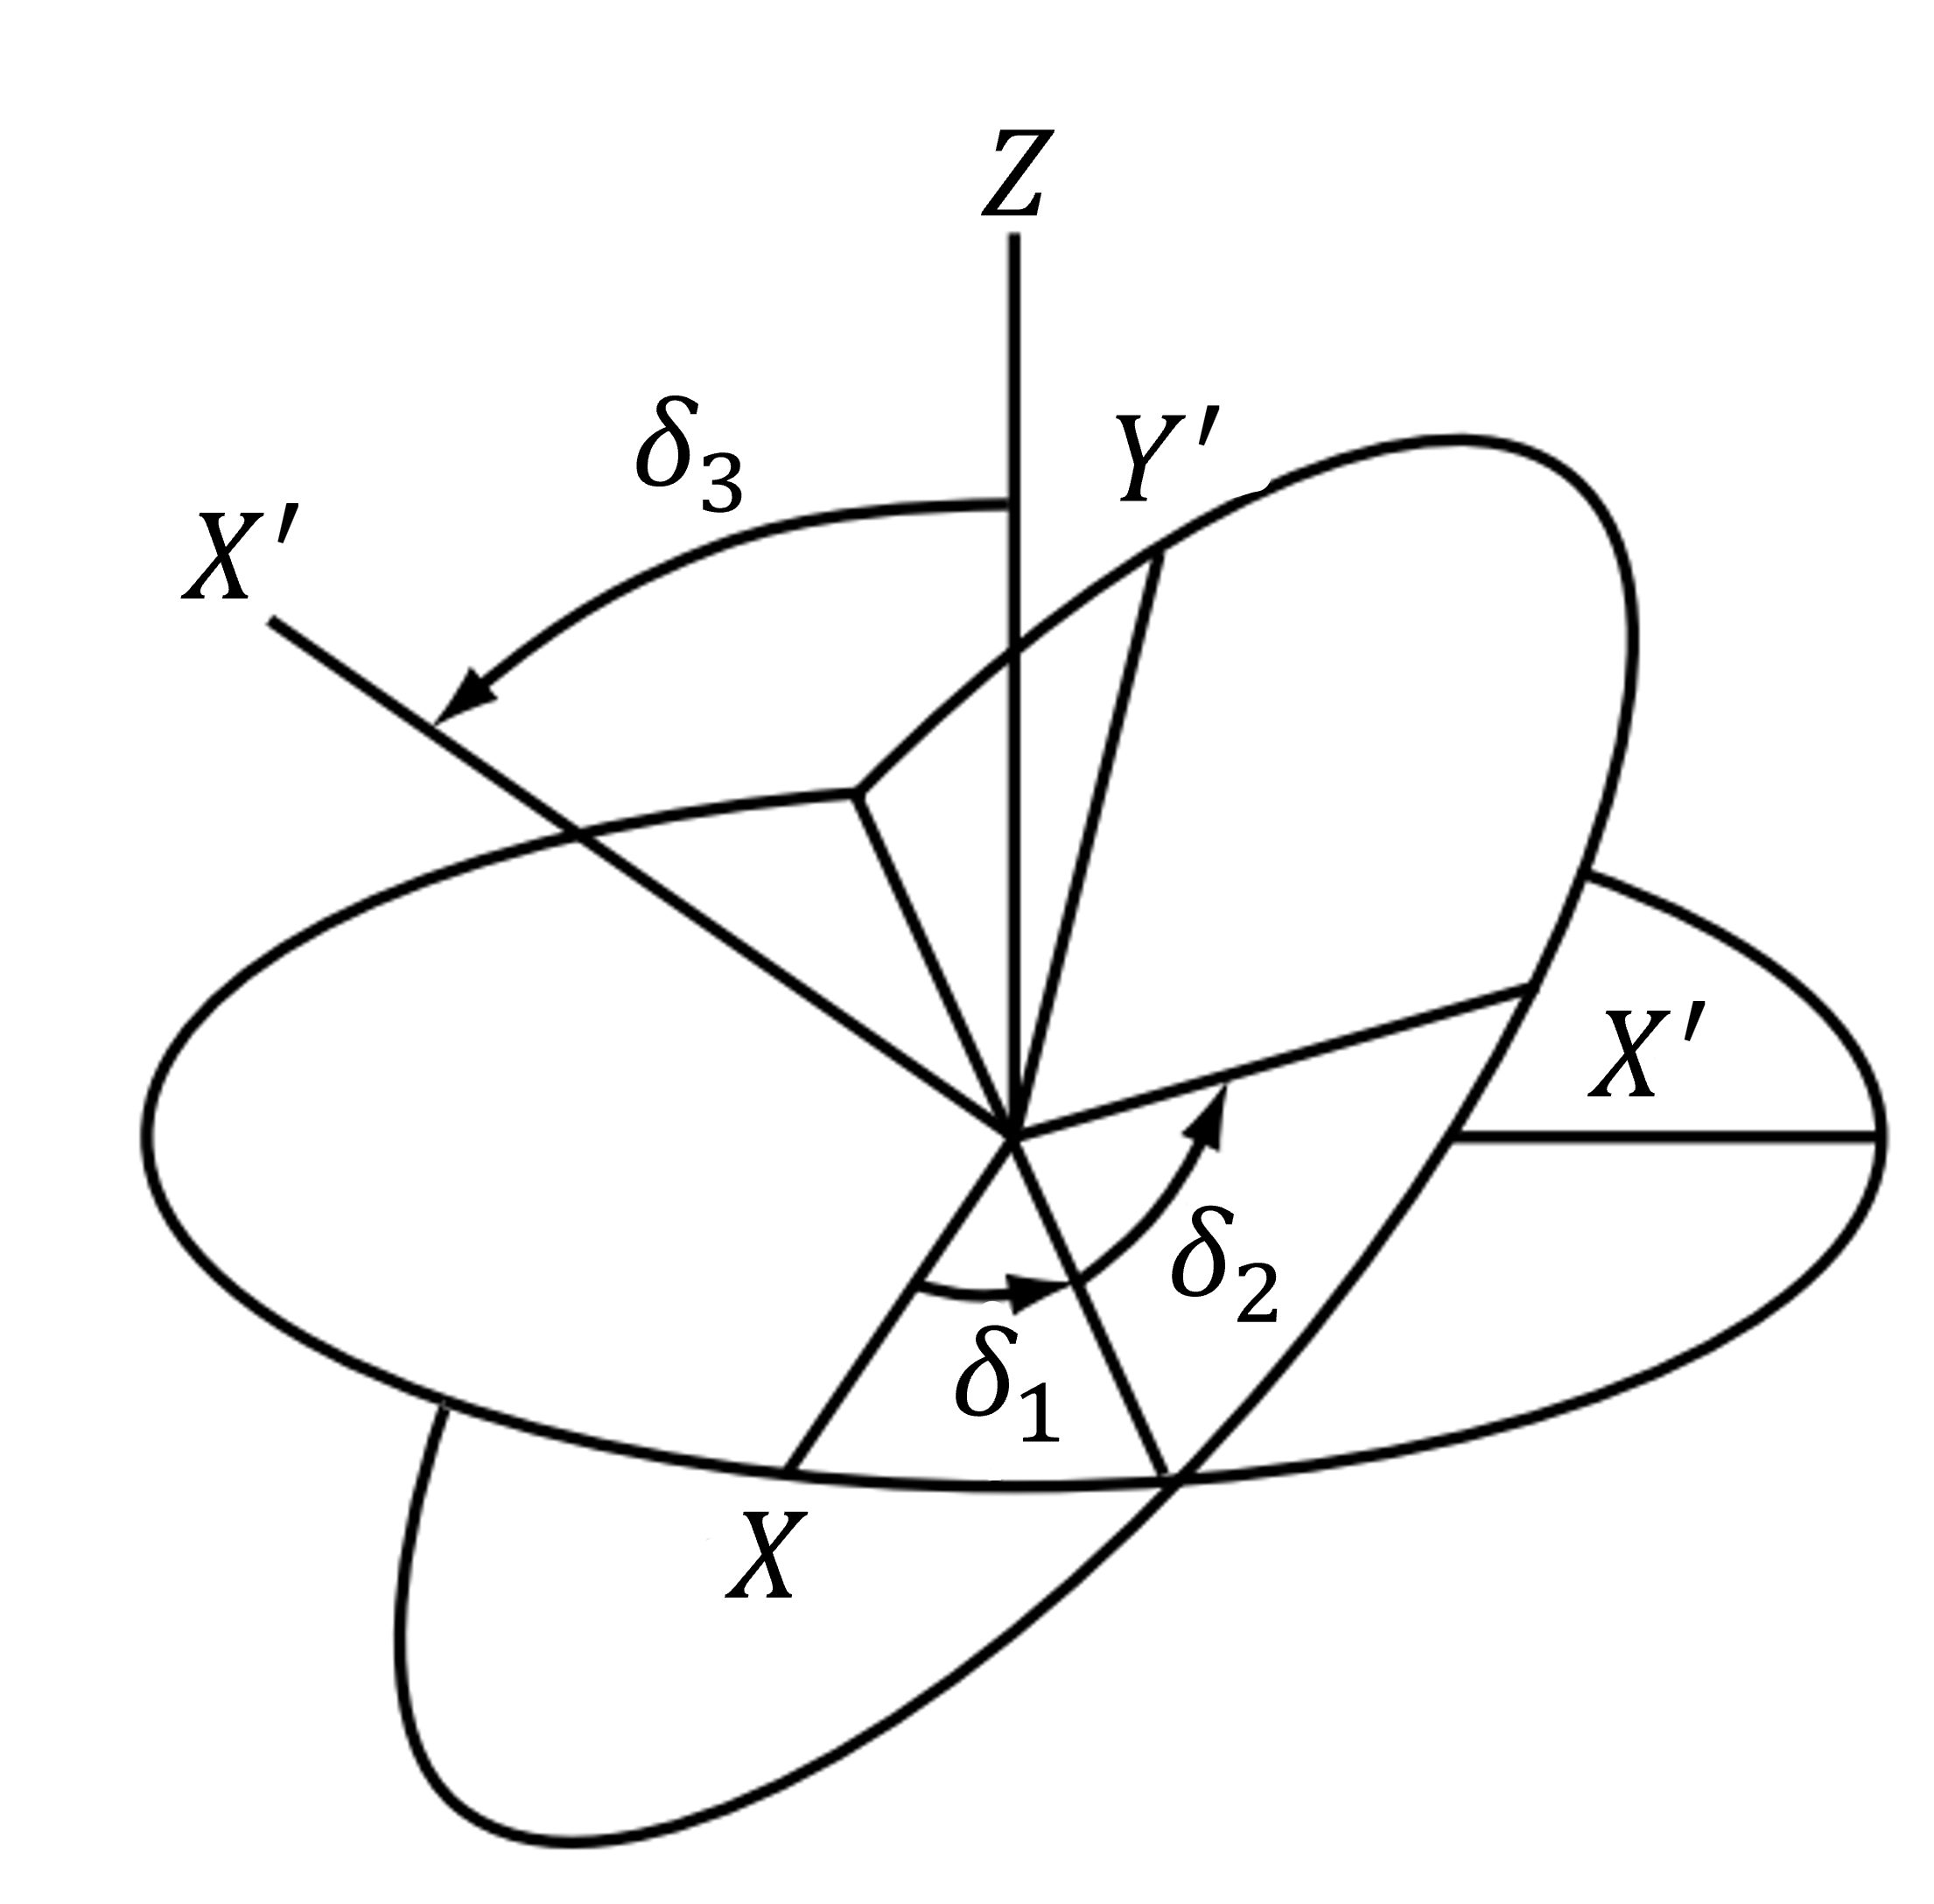
\includegraphics[width=6cm]{Figures/implementation/model/rotation_frames.png}
        \caption{Reference frame rotation Euler angles, adapted from \cite{schwab_how_2006}}
        \label{fig:rotation_frames_img}
\end{figure}

The following expressions, presented in equations \ref{eq:rotatio_zz}, \ref{eq:rotatio_yy} and \ref{eq:rotatio_xx}, define the rotation matrices of a rotation over the each of the reference axis $\hat{Z}$, $\hat{Y}$ and $\hat{X}-$axis. Also each equation present de derivetive of the rotation matrix which will be needed later on this mathematical model.

\begin{equation}
    {R o t({\hat{Z}},\eta_1)}={\left[\begin{array}{l l l}{1}&{0}&{0}\\ {0}&{c_{\eta_1}}&{-s_{\eta_1}}\\ {0}&{s_{\eta_1}}&{c_{\eta_1}}\end{array}\right]} \quad \text{and} \quad \frac{\mathrm{d}Rot(\hat{Z}, \eta_3)}{\mathrm{d}t}  = \begin{bmatrix} 0 & 0 & 0 \\ 0 & -s_{\eta_1} \dot{\eta_1} & -c_{\eta_1} \dot{\eta_1} \\ 0 & c_{\eta_1} \dot{\eta_1} & -s_{\eta_1} \dot{\eta_1} \end{bmatrix}
    \label{eq:rotatio_zz}
\end{equation}

\begin{equation}
    Rot(\hat{Y},\eta_2)=\left[\begin{array}{c c c}{{c_{\eta_2}}}&{{0}}&{{s_{\eta_2}}}\\ {{0}}&{{1}}&{{0}}\\ {{-s_{\eta_2}}}&{{0}}&{{c_{\eta_2}}}\end{array}\right] \quad \text{and} \quad \frac{\mathrm{d}Rot(\hat{Y}, \eta_2)}{\mathrm{d}t} = \left[\begin{array}{c c c}-s_{\eta_2} \dot{\eta_2} & 0 & c_{\eta_2} \dot{\eta_2} \\ 0 & 0 & 0 \\ -c_{\eta_2} \dot{\eta_2} & 0 & -s_{\eta_2} \dot{\eta_2} \end{array}\right]
    \label{eq:rotatio_yy}
\end{equation}

\begin{equation}
    Rot({\hat{ X}},{\delta_3})={\left[\begin{array}{l l l}{{{c}_{\delta_3}}}&{{-{s}_{\delta_3}}}&{{0}}\\ {{{s}_{\delta_3}}}&{{{c}_{\delta_3}}}&{{0}}\\ {{0}}&{{0}}&{{1}}\end{array}\right]} \quad \text{and} \quad \frac{\mathrm{d}Rot(\hat{X}, \delta_3)}{\mathrm{d}t} = \left[\begin{array}{c c c}
        -s_{\eta_3} \dot{\eta_3} & -c_{\eta_3} \dot{\eta_3} & 0 \\
        c_{\eta_3} \dot{\eta_3} & -s_{\eta_3} \dot{\eta_3} & 0 \\
        0 & 0 & 0
        \end{array}\right]
        \label{eq:rotatio_xx} 
\end{equation}

For the rotation matrices, it is used a simplified nomenclature where $c_{\eta_{*}}$ and $s_{\eta_{*}}$ are cosine and sine functions of the angle $\eta_{*}$. The total rotation matrix, considering the Tailt-Bryan Convention is

\begin{equation}
    Rot(\boldsymbol{\Xi})= Rot(\hat{Z},\eta_1) \cdot Rot(\hat{Y},\eta_2) \cdot Rot(\hat{X},\eta_3)
    \label{eq:total_rotation_matrix}
\end{equation}

while the derivative of the total rotation matrix is given by equation

\begin{equation}
    \frac{\mathrm{d}Rot(\boldsymbol{\Xi})}{\mathrm{d}t}= \frac{\mathrm{d}}{\mathrm{d}t} \left[Rot(\hat{Z},\eta_1) \cdot Rot(\hat{Y},\eta_2) \cdot Rot(\hat{X},\eta_3)\right].
    \label{eq:derivative_total_rotation_matrix}
\end{equation}

Proceeding with some mathematical development applying the chain rule, equation \ref{eq:derivative_total_rotation_matrix}  ca be simplified and the derivative of the total rotation matrix is


\begin{equation}
    \begin{aligned}
        \frac{\mathrm{d} \, Rot(\boldsymbol{\Xi})}{\mathrm{d}t} &= 
        \frac{\mathrm{d} Rot(\hat{Z}, \eta_1)}{\mathrm{d}t} \cdot Rot(\hat{Y}, \eta_2) \cdot Rot(\hat{X}, \eta_3) \\
        &\quad + Rot(\hat{Z}, \eta_1) \cdot \frac{\mathrm{d} Rot(\hat{Y}, \eta_2)}{\mathrm{d}t} \cdot Rot(\hat{X}, \eta_3) \\
        &\quad + Rot(\hat{Z}, \eta_1) \cdot Rot(\hat{Y}, \eta_2) \cdot \frac{\mathrm{d} Rot(\hat{X}, \eta_3)}{\mathrm{d}t}
    \end{aligned}.
    \label{eq:exp_derivative_total_rotation_matrix}
\end{equation}


Besides presenting, the previous reference frames and the relation between them, figure \ref{fig:reference_frames_img} shows another two complementary reference frames that will be further useful in \ref{sec:BET} section where a deeper insight is made about \gls{bet}. As a first introduction, the first reference frame is the blade frame, $O^b$, over which the blade's element force will be integrated to compute the total blade force, and the element reference frame, $O^e$, over which the elementary force will be calculated. A more detailed overview is done in section \ref{sec:BET} in which \gls{bet} is presented.


\subsection{System's Degrees of Freedom}

Before advance into a more advanced insight of the vehicle's laws of motion, it is importante to explain how the deegrees of freedom are. Firtsly, the translational movement in a inertial frame, due to the freefall, happens in an tri-dimensional space, once the vehicle can glide. This defines the 3-\gls{dof}. Also, the payload can rotate freely about its \gls{cg}, what means that another 3-\gls{dof} are defined once the rotation can occur along each axis. Finally, the rotor can also rotate around its hub joint cooupled at the payload's top which means three degree of freedom are needed to define the rotor's dynamic. In vector form, the state that describes the vehicle instantaneous state is 

\begin{equation}
    \aleph = \begin{bmatrix}
        x & y & z & \eta_1 & \eta_2 & \eta_3 & \zeta_1 & \zeta_2 & \zeta_3
    \end{bmatrix}^T
\end{equation}

where $x$, $y$, and $z$ are the coordinates of the vehicle's center of gravity (CG) in the inertial frame, components of $\mathbf{p}_{CG_{vehicle}}$. The vehicle's orientation is defined by Euler angles $\eta_1$, $\eta_2$, $\eta_3$ components of $\boldsymbol{\eta}$, and $\eta_1$, $\eta_2$, $\eta_3$ components of $\boldsymbol{\zeta}$ are the rotor orietation in the vehicle's frame.


%%%%%%%%%%%%%%%%%%%%%%%%%%%%%%%%%%%%%%%%%%%%%%%%%%%%%%%%%%%%%%%%%%%%%%%%
\section{7-DOF Vehicle Dynamics}
\label{section:vehicle_dynamics}

After identify the refrence frames and the vehicle's key states, it is time to introduce the strategy which easily ables to mathematically express the recovery system motion. The analysis will be separated in two parts. The first part is about vehicle the vehicle 6-\gls{dof} and its present in section \ref{section:Vehicle_Motion} and the secont part deals with the last \gls{dof}, in section \ref{section:rotor_Motion}, the rotation of the rotor. This strategy simplifies the mathematical development by decoupling the complexity of moment transfer from the rotor to the payload.


\subsection{Vehicle Motion}
\label{section:Vehicle_Motion}


The dynamics of vehicles with six degrees of freedom (6-DOF) are governed by Newton's Second Law, which relates the sum of forces (moments) acting on a body to its linear (or angular) acceleration. In this framework, define by equation \cite{cook_flight_2007}, both translational and rotational motions are considered within a three-dimensional space, making it essential for analyzing vehicles that move freely in all three spatial directions $(x, y, z)$ and rotate around their principal axes (roll, pitch, and yaw). 

For translational movement in the inertial frame, the resulting force $\mathbf{F}^i$ is given by the product of the vehicle's mass $M$ and its acceleration, $\mathbf{A}^i$, as shown in equation \ref{eq:second_law_newton}. 

\begin{equation}
    \mathbf{F}^i  = M \cdot \mathbf{A}^i
    \label{eq:second_law_newton}
\end{equation}

in the inertial frame, being the resulting force composed by the components, in the same frame, gravity, $\mathbf{F}_G^i$, the rotor force $\mathbf{F}_R^i$ and vehicle aerodynamic drag, $\mathbf{F}_{Drag}^i$,

\begin{equation}
    \mathbf{F}^i = \mathbf{F}_G^i + \mathbf{F}_R^i + \mathbf{F}_{Drag}^i.
\end{equation}

and the vehicle's mass composed by the sum of the payload's mass, $M_{payload}$, and rotor's mass , $M_{rotor}$,

\begin{equation}
    M = M_{payload} + M_{rotor}
\end{equation}


The translational velocity, $\mathbf{V}^i$,  is 

\begin{equation}
    \frac{\mathrm{d}\mathbf{V}^i}{\mathrm{d}t}\equiv  \dot{\mathbf{V}}^i = \mathbf{A}^i = \frac{1}{M} \cdot \mathbf{F}^i
\end{equation}

The reference frame is at the center of the vehicle body \gls{cg}, so there is no relative position with respect to the vehicle frame, so the position of the vechile in inertial frame, $\mathbf{P}^i$, is

\begin{equation}
    \frac{\mathrm{d}\mathbf{P}^i}{\mathrm{d}t} \equiv \dot{\mathbf{P}}^i = \mathbf{V}^i
    \label{eq:navigation_coordinates}
\end{equation}

For the rotational movement of the vehicle arounf its \gls{cg}, the second Newton's law in the vehicle frame is given by

\begin{equation}
    \mathbf{M}^i =  \frac{\mathrm{d}}{\mathrm{d}t}\mathbf{H}^i \equiv \dot{\mathbf{H}}^i
    \label{eq:total_moments_expr}
\end{equation}

where $\left[\mathbf{I}\right]^i$ is the moments vector  along each principal axis in inertial frame and $\dot{\mathbf{H}}$ is the rate of change of the angular momentum 

\begin{equation}
    \mathbf{H}^i = \left[\mathbf{I}\right]^i \boldsymbol{\omega}_{vehicle}^i
    \label{eq:angular_momentum}
\end{equation}

where $\mathbf{I}^v$ is the second moments of inertia and $\boldsymbol{\omega}_{vehicle}$ is the angular velocity in in $O^i$. Subtituting \ref{eq:angular_momentum} into \ref{eq:total_moments_expr} the equation is


\begin{equation}
    \mathbf{M}^i =  \dot{\left[\mathbf{I}\right]}^i \boldsymbol{\omega}_{vehicle}^i + \left[\mathbf{I}\right]^i\dot{\boldsymbol{\omega}}_{vehicle}^i
    \label{eq:total_moment_derivatives}
\end{equation}

Some considerations shall be made about equation \ref{eq:total_moment_derivatives}. Once the theres a degree of freedom due to the rotor rotation, the second moments of inertia matrix, $\left[\mathbf{I}\right]^i$, is not contant over time. To simplify this approach, the angular momentum $\mathbf{H}^i$, can be computed in in the vehicle frame, $O^v$, for equation \ref{eq:total_moments_expr}, as

\begin{eqnarray}
    \mathbf{M}^i =  \dot{\mathbf{H}}^v + \boldsymbol{\Omega}_{REF} \times \mathbf{H}^v
\end{eqnarray}

and then

\begin{equation}
    \mathbf{M}^i = \frac{\mathrm{d}}{\mathrm{d}t} \left(\left[\mathbf{I}\right]^v \boldsymbol{\omega}_{\text{vehicle}}^v\right) + \boldsymbol{\Omega}_{REF} \times \left(\left[\mathbf{I}\right]^v \boldsymbol{\omega}_{\text{vehicle}}^v\right)
\end{equation}

Once $\dot{\left[\mathbf{I}\right]}^v = 0$, then

\begin{equation}
    \mathbf{M}^i =\left[\mathbf{I}\right]^v \dot{\boldsymbol{\omega}}_{vehicle}^v + \boldsymbol{\Omega}_{REF} \times \left(\left[\mathbf{I}\right]^v \boldsymbol{\omega}_{\text{vehicle}}^v\right)
\end{equation}


\textcolor{red}{fiquei aquiiiiiiiii na equação de cima}

with a constant $\mathbf{I}^r$ once the rotor is always aligned withe $O^r$ and the cilinder does not made any change in $\mathbf{I}^r$. The total moment, $\mathbf{M}^r$, is 

\begin{equation}
    \mathbf{M}^r = \mathbf{M}_G^r + \mathbf{M}_R^r + \mathbf{M}_{Drag}^r.
\end{equation}

Where $\mathbf{M}_G^r$ is the moment caused from gravity in each point mass force, $\mathbf{M}_R^r$ from the rotor force and $\mathbf{M}_{Drag}^r$ from the vehicle aerodynamic drag. The vehicle's angular velocity, $\boldsymbol{\omega}^r_{vehicle}$, in $O^r$ is

\begin{equation}
    \frac{\mathrm{d}\boldsymbol{\omega}^r_{vehicle}}{\mathrm{d}t} \equiv \boldsymbol{\dot{\omega}}^r_{vehicle} = \boldsymbol{\chi}^r_{vehicle} = (\mathbf{I}^r)^{-1} \mathbf{M}^r.
    \label{eq:angular_acceleration_inRotor}
\end{equation}

However, the interest is the angular acceleration in the $O^v$. So, to obtain the anguar acceleration in $O^v$

\begin{equation}
    \boldsymbol{\chi}^r_{vehicle} = \boldsymbol{R}^*_{v \rightarrow r} \boldsymbol{\chi}^v_{vehicle} \implies \boldsymbol{\chi}^v_{vehicle} = \left(\boldsymbol{R}^*_{v \rightarrow r}\right)^{-1} \boldsymbol{\chi}^r_{vehicle}
    \label{eq:angular_acceleration_inVehicle}
\end{equation}

Using equation \ref{eq:angular_acceleration_inVehicle} into equation \ref{eq:angular_acceleration_inRotor}, the vehicles angular acceleration around its \gls{cg} is

\begin{equation}
    \boldsymbol{\dot{\omega}}^v_{vehicle} = \left(\boldsymbol{R}^*_{v \rightarrow r}\right)^{-1} (\mathbf{I}^r)^{-1} \mathbf{M}^r.
\end{equation}


and the angular position which shall be considered as a rotation of $O^v$ in $O^i$, so


\begin{equation}
    \frac{\mathrm{d}\boldsymbol{\Xi}^i_{vehicle}}{\mathrm{d}t} \equiv \dot{\boldsymbol{\Xi}}^i_{vehicle} = \boldsymbol{\omega}^i_{vehicle}
\end{equation}

The angular velocity was previously presented in \ref{eq:angular_acceleration_inVehicle}, but needs to be written in $O^i$ to compute vehicle orientation considerting euler angles the Euler angles. Then,

\begin{equation}
    \boldsymbol{\omega}^v_{vehicle} = \boldsymbol{R}^*_{i \rightarrow v} \boldsymbol{\omega}^i_{vehicle} \implies \boldsymbol{\omega}^i_{vehicle} = \left(\boldsymbol{R}^*_{i \rightarrow v}\right)^{-1} \boldsymbol{\omega}^v_{vehicle} 
\end{equation}

and finally the vehicle's orientation equation is

\begin{equation}
    \dot{\boldsymbol{\Xi}}^i_{vehicle} = \left(\boldsymbol{R}^*_{i \rightarrow v}\right)^{-1} \boldsymbol{\omega}^v_{vehicle} 
\end{equation}

\subsection{Rotor Motion}
\label{section:rotor_Motion}

To desbribe the rotor motion, a very simple simplication can be made once only one degree of freedom is defined. The rotation is about the vertical axis either for $O^v$ and for $O^r$. Also, the only force, needed to be considered in this dynamic, is the in-plane propulsive force generated during the phenomena of autorotation.

The rotor montion is defined by a single equation and can be deduced as for the vehicle´s rotation throw its \gls{cg}. The velocity in $O^v$ of the rotor is 


\begin{equation}
    \frac{\mathrm{d}\omega^v_{rotor}}{\mathrm{d}t} \equiv \dot{\omega}^v_{rotor} \equiv \dot{\omega}^r_{rotor} = \frac{1}{I^r_{x_{rotor}}} M^r_{rotor}
\end{equation}

The position can be simply computed as

\begin{equation}
    \frac{\mathrm{d}\Psi^v_{rotor}}{\mathrm{d}t} \equiv \dot{\Psi}^v_{rotor} = \omega^r_{rotor} 
\end{equation}

\subsection{Full system}

To caracterize the full system of the 7-\gls{dof} model, one can expand the variables used, considering for the vehicles movement. Starting with the translational movement

\begin{equation}
    \mathbf{V}^i = \begin{bmatrix} u \\ v \\ w \end{bmatrix}
    \quad \text{and} \quad 
    \mathbf{P}^i = \begin{bmatrix} X \\ y \\ z \end{bmatrix}
\end{equation}

For the vechile's rotation

\begin{equation}
    \boldsymbol{\omega}^v_{vehicle} = \begin{bmatrix} p \\ q \\ r \end {bmatrix}
    \quad \text{and} \quad
    \mathbf{\Xi}^v_{vehicle} = \begin{bmatrix} \delta_1 \\ \delta_2 \\ \delta_3 \end {bmatrix}
\end{equation}

For the forces and moments

\begin{equation}
    \mathbf{F}^i = \begin{bmatrix} F_x \\ F_y \\ F_z \end {bmatrix}
    \quad \text{and} \quad
    \mathbf{M}^r = \begin{bmatrix} M_x \\ M_y \\ M_z \end {bmatrix}
\end{equation}


\textcolor{blue}{translação}

\begin{equation}
    \begin{bmatrix} \dot{u} \\ \dot{v} \\ \dot{w} \end{bmatrix} = \frac{1}{M} \begin{bmatrix} F_x \\ F_y \\ F_z \end {bmatrix}
\end{equation}


\begin{equation}
    \begin{bmatrix} \dot{x} \\ \dot{y} \\ \dot{z} \end{bmatrix} = \begin{bmatrix} u \\ v \\ w \end{bmatrix}
\end{equation}


\textcolor{blue}{rotação}

\begin{equation}
    \begin{bmatrix} \dot{p} \\ \dot{q} \\ \dot{r} \end {bmatrix} = \left[\boldsymbol{R}^*_{v \rightarrow r}\left(\Psi\right)\right]^{-1} (\mathbf{I}^r)^{-1} \begin{bmatrix} M_x \\ M_y \\ M_z \end {bmatrix}
\end{equation}

\begin{equation}
    \begin{bmatrix} \dot{\delta_1} \\ \dot{\delta_2} \\ \dot{\delta_3} \end{bmatrix} = \left[\boldsymbol{R}^*_{i \rightarrow v} \left(\delta_1, \delta_2, \delta_3 \right)\right]^{-1} \begin{bmatrix} p \\ q \\ r \end{bmatrix}
\end{equation}

\textcolor{blue}{para o rotor}

\begin{equation}
    \dot{\omega}^r_{rotor} = \frac{1}{I^r_{x_{rotor}}} M^r_{rotor}
\end{equation}

\begin{equation}
    \dot{\Psi}^v_{rotor} = \omega^r_{rotor} 
\end{equation}


\subsection{Moment of Inertia}


\begin{equation}
    \mathbf{I}=\left[\begin{array}{c c c}{{I_{x x}}}&{{-I_{x y}}}&{{-I_{x z}}}\\ {{-I_{x y}}}&{{I_{y y}}}&{{I_{-y z}}}\\ {{-I_{x z}}}&{{-I_{y z}}}&{{I_{z z}}}\end{array}\right]
\end{equation}

\begin{equation}
    I_{xx} = \smallint  \left( y^2 + z^2 \right) \mathrm{d}m \quad \text{and} \quad I_{yy} = \smallint  \left( x^2 + z^2 \right) \mathrm{d}m \quad \text{and} \quad I_{zz} = \smallint  \left( x^2 + y^2 \right) \mathrm{d}m
\end{equation}


\begin{equation}
    I_{xy} = \smallint  xy \, \mathrm{d}m \quad \text{and} \quad I_{xz} = \smallint  xz \, \mathrm{d}m \quad \text{and} \quad I_{yz} = \smallint  yz \, \mathrm{d}m
\end{equation}



%%%%%%%%%%%%%%%%%%%%%%%%%%%%%%%%%%%%%%%%%%%%%%%%%%%%%%%%%%%%%%%%%%%%%%%%

\section{Blade Element Theory (BET)}
\label{sec:BET}

The Blade Element Theory (BET) is a simplefied modern model to study the rotor performance \cite{leishman_principles_2006}. With \gls{bet}, it is possible to make predictions about radia and azimuthal aerodynamic load distributions over the rotor disk. Its principel is based in a quasi-2D airfoils blade section which generate the aerodynamic forces and moments that shall be integrated over the blade length. With \gls{bet} methodology is possible to performe a rotor's first designing shape stage in terms of blade geometry.

\begin{figure}[!htb]
    \centering
        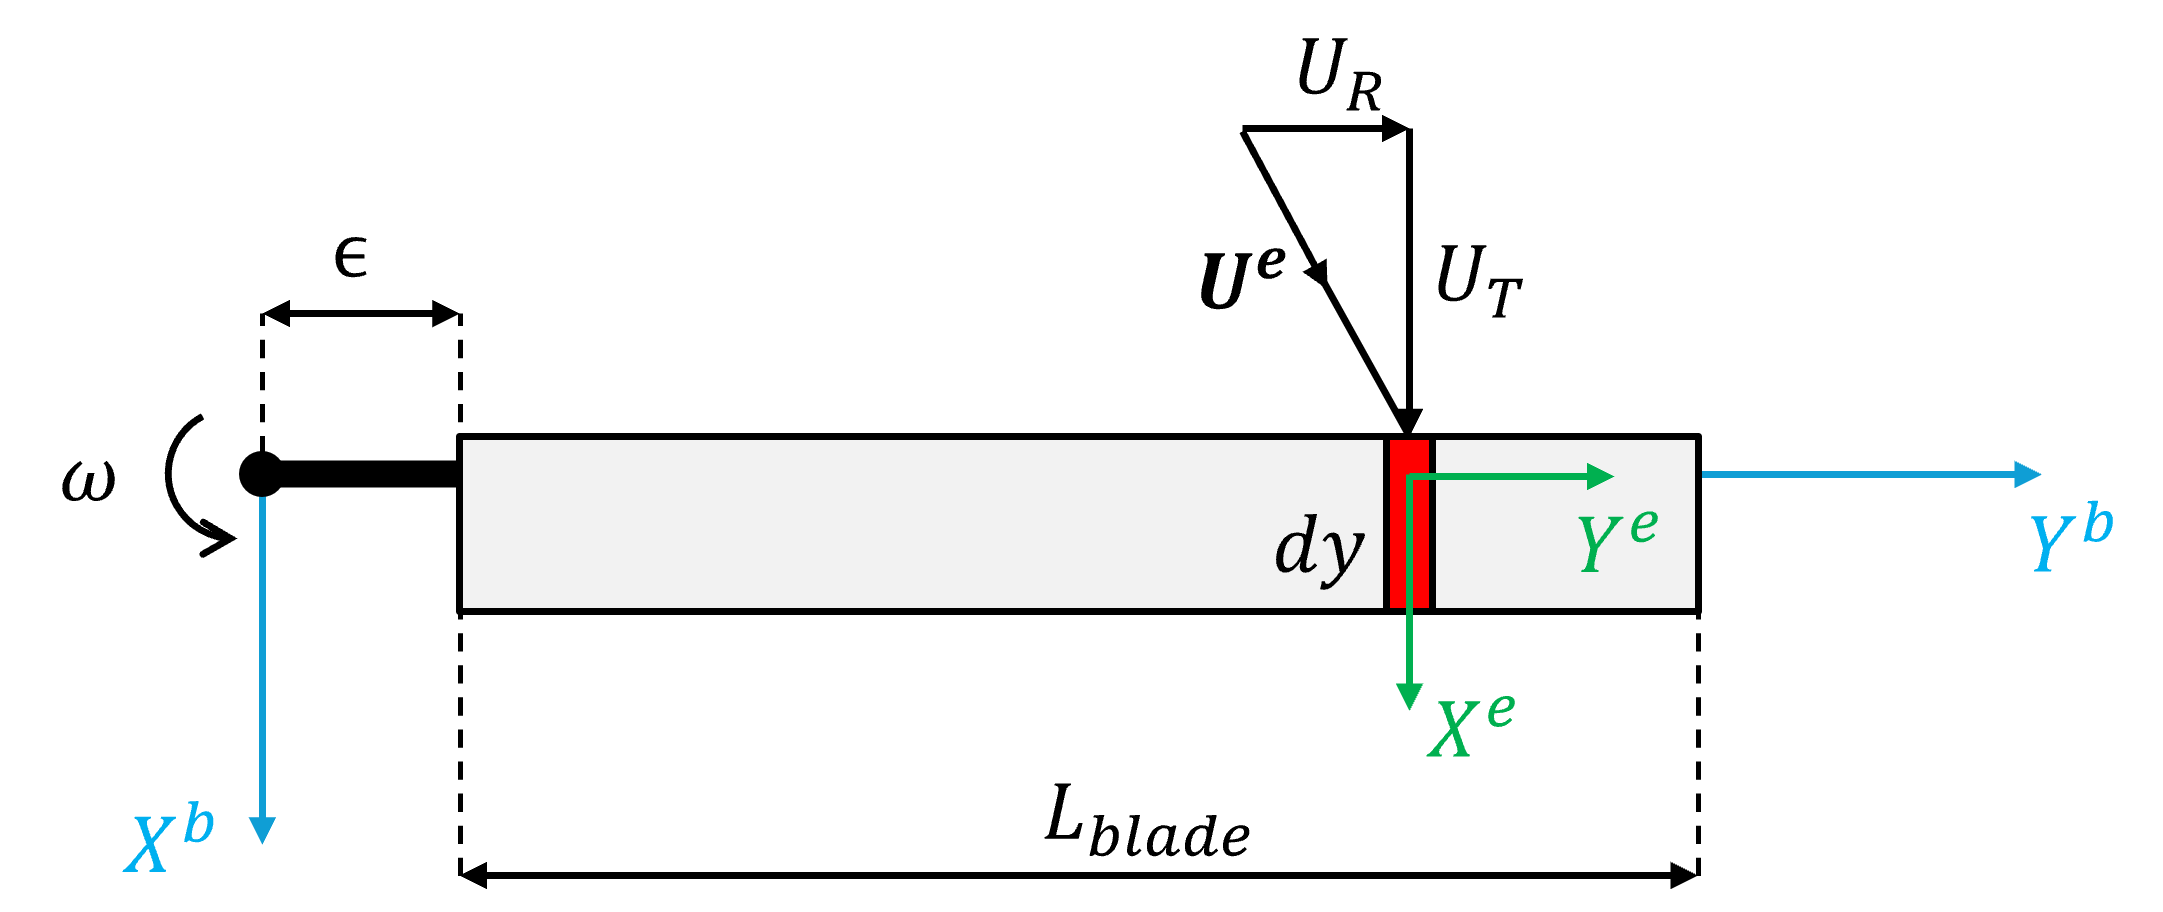
\includegraphics[width=9cm]{Figures/implementation/bet/blade_model.png}
        \caption{Image \textcolor{blue}{falta trocar as referencias dos eixos}}
\end{figure}


\subsection{Blade forces and moments}
\label{section:bem_forces_moments}

\textcolor{blue}{Forces in Element Frame}

\begin{equation}
    (\mathrm{d}L^{e})_n = \frac{1}{2} \rho \cdot   \|  \left( \mathbf{V}^e \right)_n \| ^2 dy
    \label{eq:elementary_lift}
\end{equation}

\begin{equation}
    (\mathrm{d}D^{e})_n = \frac{1}{2} \rho \left[ C_d \right] \|  \left( \mathbf{V}^e \right)_n \| ^2 dy
    \label{eq:elementary_drag}
\end{equation}

\textcolor{blue}{Blade Force in Blade Frame}

\begin{equation}
    \left(\mathbf{T}^{b}\right)_m = \int_\epsilon^R \left( \mathrm{d}\mathbf{F}^{e}\right)_n \, \mathrm{d}y
\end{equation}

\begin{equation}
    \left(\mathbf{T}^{b}\right)_m = \int_\epsilon^R \left(\mathbf{r}^e \right)_n \times \left( \mathrm{d}\mathbf{F}^{e}\right)_n \, \mathrm{d}y
\end{equation}


\begin{equation}
    \left(\mathbf{r}^e \right)_n = \begin{bmatrix} 0 & n \cdot \left(\frac{L_{rotor}}{N_e}\right) & 0 \end{bmatrix}^T
\end{equation}



\textcolor{blue}{Blade Force in Rotor Frame}

\begin{figure}[!htb]
    \centering
        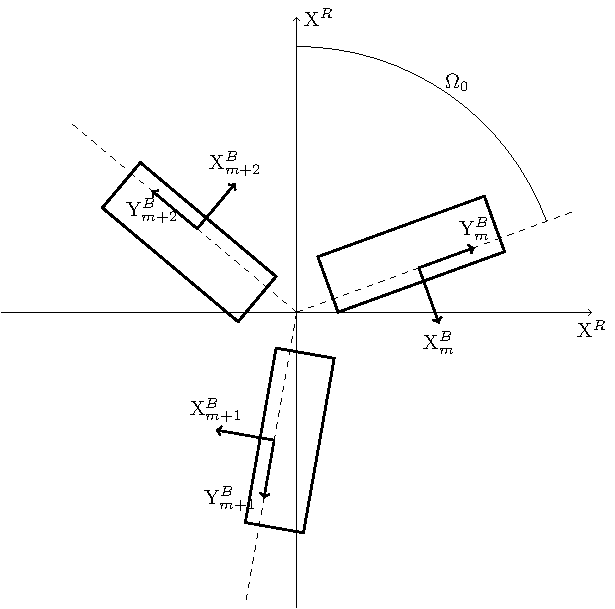
\includegraphics[width=8cm]{Figures/implementation/bet/blade_forces/multiple_blades_reference.pdf}
        \caption{Image \textcolor{blue}{falta trocar as referencias dos eixos}}
\end{figure}

\begin{equation}
    \left(\mathbf{F}^{r}\right)_m = Rot(\hat{\mathbf{z}}, \Omega_m) \cdot \left(\mathbf{F}^{b}\right)_m = Rot(\hat{\mathbf{z}}, \Omega_m) \cdot \int_\epsilon^R \left( \mathrm{d}\mathbf{F}^{e}\right)_n \, \mathrm{d}y
\end{equation}

\begin{equation}
    \left(\mathbf{T}^{r}\right)_m = Rot(\hat{\mathbf{z}}, \Omega_m) \cdot \left(\mathbf{T}^{b}\right)_m = Rot(\hat{\mathbf{z}}, \Omega_m) \cdot \int_\epsilon^R \left(\mathbf{r}^e \right)_n \times \left( \mathrm{d}\mathbf{F}^{e}\right)_n \, \mathrm{d}y
\end{equation}

%\begin{equation}
%	\Omega_m = \Omega_{0} +  m \cdot \frac{2\pi}{N_b}, \quad m \in \{0,1,2,\dots \}
%\end{equation}

\textcolor{blue}{Total Rotor Force and Torque in Rotor Frame}

\begin{equation}
    \mathbf{F}^{r} = \sum_m \left(\mathbf{F}^{r}\right)_m
\end{equation}


\begin{equation}
    \mathbf{T}^{r} = \sum_m \left(\mathbf{T}^{r}\right)_m 
\end{equation}


\textcolor{blue}{Forces in Blade Frame}

\begin{figure}[!htb]
    \centering
    \begin{minipage}{0.45\textwidth}
        \centering
        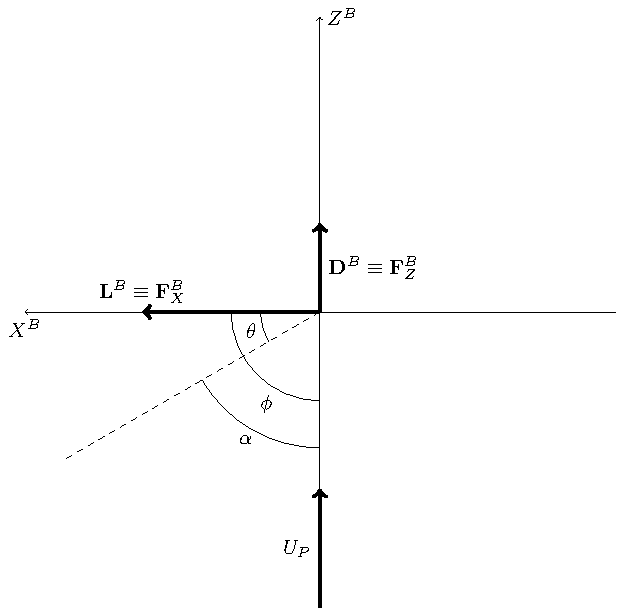
\includegraphics[width=\linewidth]{Figures/implementation/bet/blade_forces/blade_element_forces_1.pdf} % Replace with your image file
        \caption{Image 1}
    \end{minipage}
    \hfill
    \begin{minipage}{0.45\textwidth}
        \centering
        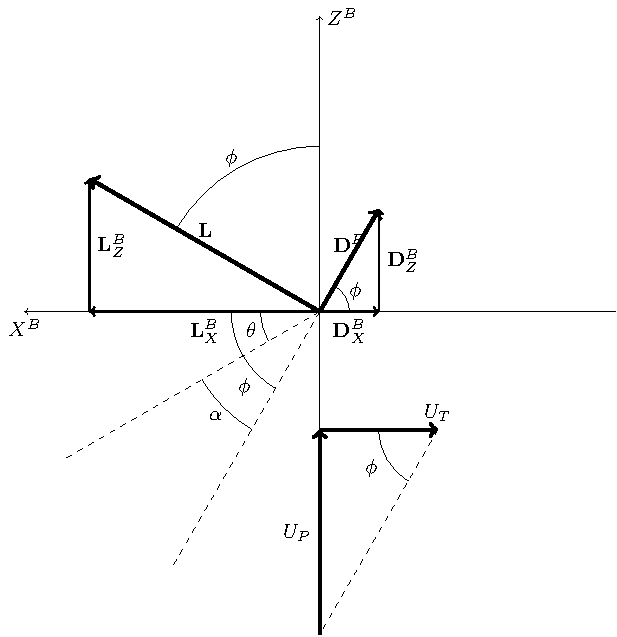
\includegraphics[width=\linewidth]{Figures/implementation/bet/blade_forces/blade_element_forces_2.pdf} % Replace with your image file
        \caption{Image 2}
    \end{minipage}
    \vfill
    \begin{minipage}{0.45\textwidth}
        \centering
        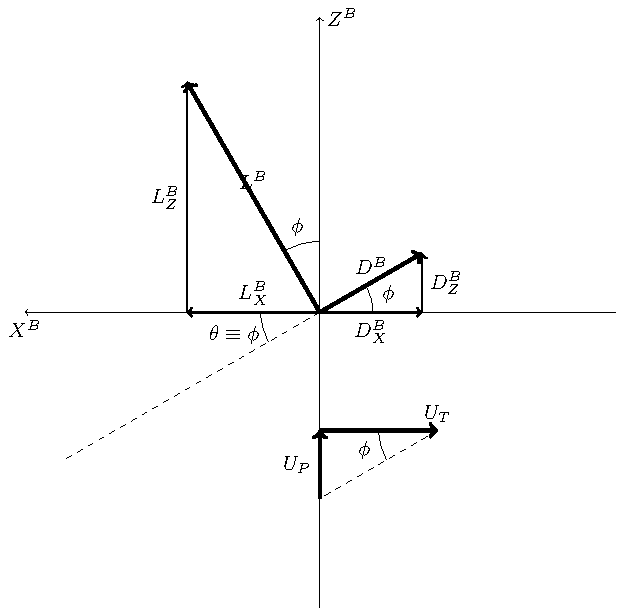
\includegraphics[width=\linewidth]{Figures/implementation/bet/blade_forces/blade_element_forces_3.pdf} % Replace with your image file
        \caption{Image 3}
    \end{minipage}
    \hfill
    \begin{minipage}{0.45\textwidth}
        \centering
        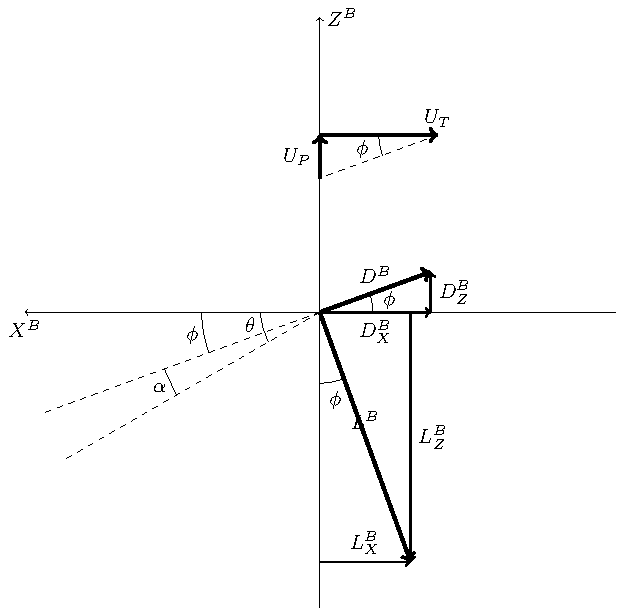
\includegraphics[width=\linewidth]{Figures/implementation/bet/blade_forces/blade_element_forces_4.pdf} % Replace with your image file
        \caption{Image 4}
    \end{minipage}
    \caption{2x2 Grid of Images \textcolor{blue}{falta trocar as referencias dos eixos}}
\end{figure}


\begin{figure}[!htb]
    \centering
    \begin{minipage}{0.45\textwidth}
        \centering
        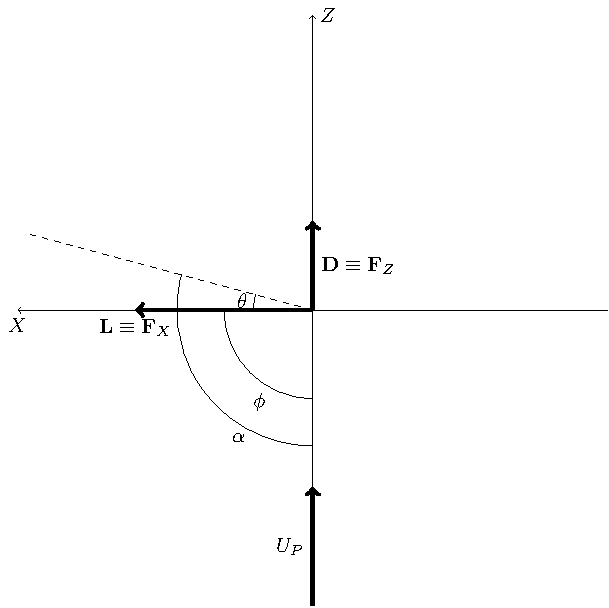
\includegraphics[width=\linewidth]{Figures/implementation/bet/blade_forces/blade_element_forces_5.pdf} % Replace with your image file
        \caption{Image 1}
    \end{minipage}
    \hfill
    \begin{minipage}{0.45\textwidth}
        \centering
        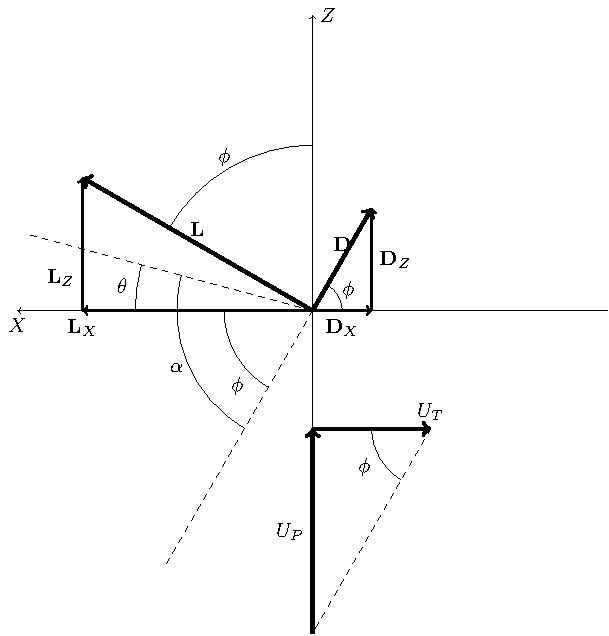
\includegraphics[width=\linewidth]{Figures/implementation/bet/blade_forces/blade_element_forces_6.pdf} % Replace with your image file
        \caption{Image 2}
    \end{minipage}
    \caption{1x2 Grid of Images \textcolor{blue}{falta trocar as referencias dos eixos}}
\end{figure}

\subsection{Velocities}

\textcolor{blue}{Element Velocity in  Element Frame}

\begin{equation}
    \mathbf{V}^i = Rot(E_A)  \mathbf{V}^v \implies \mathbf{V}^v = Rot(E_A)^{-1} \mathbf{V}^i
\end{equation}

$$
    \text{Element Velocity} = \text{Vehicle Translation} + \text{Vehicle Rotation } + \text{Rotor Rotation} + \text{Induced Velocity}
$$


\begin{equation}
    \left( \mathbf{V}^e \right)_n =  \underbrace{\boldsymbol{V}^e_T}_\text{Vehicle Translation} + \underbrace{\left(\mathbf{r}_{CM}\right)_n \times \boldsymbol{\omega}^v_{vehicle}}_\text{Vehicle Rotation } + \underbrace{\left(\mathbf{r}^e\right)_n \times \boldsymbol{\omega}^r_{rotor}}_\text{Rotor Rotation} + \underbrace{\boldsymbol{v}_{i}^r}_\text{Induced Velocity}
\end{equation}


\textcolor{blue}{Velocidade de translação}



\begin{equation}
    \mathbf{P}^e =  \boldsymbol{R}^*_{v \rightarrow e} \mathbf{P}^v 
\end{equation}

\begin{equation}
    \mathbf{V}^e_T \equiv \frac{\mathrm{d}\mathbf{P}^e}{\mathrm{d}t} =  \frac{\mathrm{d}}{\mathrm{d}t} \left(\boldsymbol{R}^*_{v \rightarrow e} \mathbf{P}^v \right) \implies  \mathbf{V}^e_T = \boldsymbol{\dot{R}}^*_{v \rightarrow e} \mathbf{P}^v + \boldsymbol{R}^*_{v \rightarrow e} \dot{\mathbf{P}}^v
\end{equation}

\begin{equation}
    \mathbf{V}^e_T = \dot{\boldsymbol{R}}^*_{v \rightarrow e} \mathbf{P}^v + \boldsymbol{R}^*_{v \rightarrow e} \mathbf{V}^v
\end{equation}

\subsubsection{Induced Velocity}

\textcolor{blue}{Windmill Break State}

\begin{equation}
    {\frac{v_{i}}{v_{h}}}=-\left({\frac{V_{c}}{2v_{h}}}\right)-{\sqrt{\left({\frac{V_{c}}{2v_{h}}}\right)^{2}-1}},
\end{equation}

\textcolor{blue}{Vortex Ring State}

\begin{equation}
    \frac{v_{i}}{v_{h}}=\kappa+k_{1}\left(\frac{V_{c}}{v_{h}}\right)+k_{2}\left(\frac{V_{c}}{v_{h}}\right)^{2}+k_{3}\left(\frac{V_{c}}{v_{h}}\right)^{3}+k_{4}\left(\frac{V_{c}}{v_{h}}\right)^{4}
\end{equation}

\textcolor{blue}{Como o $v_i$ é escrito no referencial do rotor, e o referencial do rotor está alinha com o referencial do veiculo, então não é necessário converter entre referencais, apenas criar um vetor com componente vertical. Como a velocidade induzida é para a parte de baixo do rotor, então fica com componente negativa}

\begin{equation}
   \boldsymbol{v}_{i}^v \equiv \boldsymbol{v}_{i}^r = \begin{bmatrix} 0 & 0 & -v_i \end{bmatrix}^T
\end{equation}


\section{Reynolds Number}

\begin{eqnarray}
    Re = \frac{\rho \norm{\boldsymbol{V}} c}{\mu}
    \label{eq:reynolds_number}
\end{eqnarray}

\section{AERODAS Model}
\label{section:aerodynamic_model}

\textcolor{blue}{Motivar a necessidade de haver um modelo aerodinâmico}

As seen in section \ref{section:bem_forces_moments}, the \gls{bet} is a based model, in short words, defined a sum of elementary 2D airfoil setions. Then its crucial for its implementation a computational method to obtain $\left[ C_l \right]$ and $\left[ C_d \right]$ for 2D airfoils, in equations \ref{eq:elementary_lift} and \ref{eq:elementary_drag}.

\textcolor{blue}{questões computacionais}

Also \gls{bet} has critical consideration rather the number of elements used to define a blade. The higher the number of elements, the higher the number of calculations needed to be perform a rotor analysis. This means that for a time-dependent model as a free-fall considered in this work, more critical it is, in term of computational time, to perform any simulation. So a fast model should be used.

\textcolor{blue}{altos angulos de ataque}

For choosing a airfoil analysis, one must consider the rotor dynamics. In this study, the rotor is under the phenomena of autorotation which has its displacement mainly in descent direction, then some considerations should be made about the angles of attack. On blade's root, the angular velocity is smaller when compared to the blade's tip. Meaning, the inflow angle is mainly composed by a vertical component rather than a horizontal component. So, a wider range of angles of attack should be considered. Also, if it is considered a pure vertical descent mode and small rotor angular velocity, the angles of attack while certainly be near 90$^{\circ}$ meaning that the rotor will work on a stall model. A reference to the pitch angle, $\theta$, and the blade twist should be made, however for thin airfoils it is known that for angles near 20~30$^{\circ}$, depending on thickness and camber, the airfoils starts to operate as a flate plate on stall mode, with completely separate boundary layers.

\textcolor{blue}{apresentação do aerodas}

This consideration are needed in other aerodynamic applications of rotors operating in high angles of attack, namely in wind turbines. So, David A. Spera developed an aerodynamic model \cite{spera_models_2008} naned AERODAS, for to predict lift and drag coefficients for stallel and unstalled airfoils. 

The development of horizontal-axis wind turbines is described in this article as a result of a Department of Energy-sponsored and NASA-led federal effort that ran from 1973 to 1995. This study develops an empirical model for airfoil lift and drag by fitting test data with algebraic equations, rather than using aerodynamic theory. It includes a wide range of conditions such as different airfoils, Reynolds numbers, and angles of attack, and also models circular cylinders and thin plates. Key improvements include expanding the test data set to cover more airfoils and configurations. Unlike previous models, it uses empirical equations derived from actual airfoil behavior at high angles of attack in the post-stall regime, rather than assuming flat plate behavior. 

The model also considers airfoil thickness in addition to aspect ratio and angle of attack. Its accuracy is evaluated by calculating the mean and standard deviation of the lift and drag data across various airfoils. Finally, the model is applied in Blade Element Momentum (BEM) analysis to predict wind turbine power and fan performance, and its results are compared with measured data to evaluate its effectiveness.

\textcolor{blue}{modelo}

Going deeper into the mathematical prespective, the AERODAS model main goal is to get the lift, $C_l$, and drag,$C_d$, curves as function of angle of attack, $\alpha$. Figure \ref{fig:aerodas_functions} presents the considered curves and highlight the major considerations about the model.

\begin{figure}[!htb]
    \centering
    \subfloat[AERODAS model lift coefficient,$C_l$, as functio of angle of attack,$\alpha$, from \cite{spera_models_2008}\label{fig:aerodas_cl}]{
        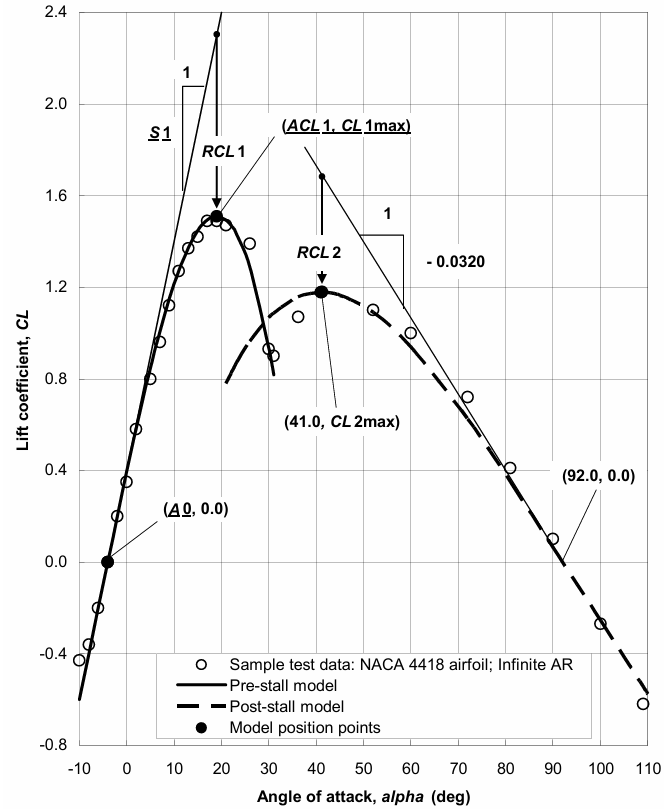
\includegraphics[height=8.5cm]{Figures/implementation/bet/aerodas/aerodas_cl_model.png}
    }\hfill
    \subfloat[AERODAS model drag coefficient,$C_d$, as functio of angle of attack,$\alpha$, from \cite{spera_models_2008}\label{fig:aerodas_cd}]{
        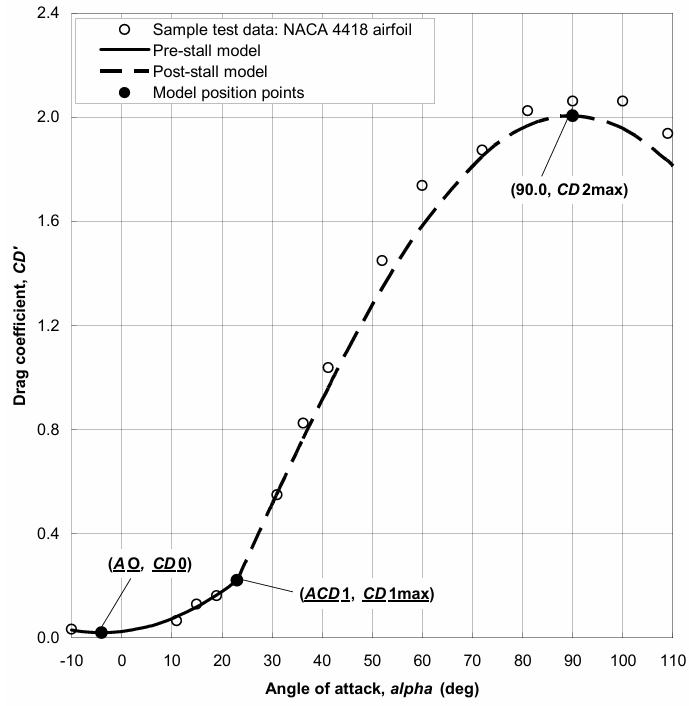
\includegraphics[height=8.5cm]{Figures/implementation/bet/aerodas/aerodas_cd_model.png}
    }
    \caption{AERODAS model curves}
    \label{fig:aerodas_functions}
\end{figure}

From \cite{spera_models_2008}, the main equations for the model are presented in table \ref{tab:aerodas_key_equation}. The key point of AERODAS model is separate the lift and drag curve with equations for pre-stall and post stall regimes. 

\textcolor{blue}{equações de lift}

For lift it is defined mathematical expressions for pre-stall, $CL1$, considering the Spera \cite{spera_models_2008} uses a proposed model by Viterna, where it consideres a linear variation for the lift coefficient, $S1$, and while $\alpha$ increases approaching the stall angle $ACL1$, the function uses a reduction from extension of linear segment of lift curve to $CL1_{max}$ (maxima $CL$ value, before stall), $RCL1$, 

% Please add the following required packages to your document preamble:
% \usepackage{multirow}
\begin{table}[!htb]
    \centering
    \renewcommand{\arraystretch}{2.5} % Aumenta o espaço entre as linhas
    \footnotesize % Reduz o tamanho da fonte (use \footnotesize ou \scriptsize se quiser menor ainda)
    \begin{tabular}{llll}
        \hline
        Mode                        & Coefficient                                     & Condition                                   & Equation                                                                                                                    \\ \hline
        \multirow{4}{*}{Pre-stall}  & \multicolumn{1}{c}{\multirow{2}{*}{Lift $CL1$}} & $\alpha \geq A0$                            & $C L1=S1\cdot\left(\alpha-A0\right)-R C L1\left(\frac{\alpha-A0}{A C L1-A0}\right)^{N1}$                                    \\
                                    & \multicolumn{1}{c}{}                            & $\alpha < A0$                               & $CL1=S1\cdot(\alpha-A0)+R C L1\left(\frac{A0-\alpha}{A C L1-A0}\right)^{N1}$                                                \\ \cline{2-4} 
                                    & \multirow{2}{*}{Drag $CD1$}                     & $(2 A0 - ACD1) \leq \alpha \leq ACD1$       & $C D1=C D0+\left(C D1\operatorname*{max}-C D0\right)\left({\frac{\alpha-A0}{A C D1-A0}}\right)^{M}$                         \\
                                    &                                                 & $\alpha < (2 A0 - ACD1)$ or $\alpha > ACD1$ & $CD1=0$                                                                                                                     \\ \hline
        \multirow{7}{*}{Post-stall} & \multicolumn{1}{c}{\multirow{4}{*}{Lift $CL2$}} & $0 < \alpha < ACL1$                         & $CL2=0$                                                                                                                     \\
                                    & \multicolumn{1}{c}{}                            & $ACL1 \leq \alpha \leq 92^{\circ}$          & $CL2=-0.032\left(\alpha-92.0\right) - RCL2\cdot\left({\frac{92.0-\alpha}{51.0}}\right)^{N2}$                                \\
                                    & \multicolumn{1}{c}{}                            & $\alpha > 92^{\circ}$                       & $CL2=-0.032\left(\alpha-92.0\right) + RCL2 \cdot \left(\frac{\alpha-92.0}{51.0}\right)^{N2}$                                \\
                                    & \multicolumn{1}{c}{}                            & $\alpha < 0$                                & $CL2[\alpha] = - CL2[-\alpha + 2 \cdot A0]$                                                                                 \\ \cline{2-4} 
                                    & \multirow{3}{*}{Drag $CD2$}                     & $(2A0-ACL1) \leq \alpha \leq ACL1$          & $CD2 = 0$                                                                                                                   \\
                                    &                                                 & $\alpha \geq ACD1$                          & $\begin{aligned}CD2 = CD1_{max}+\left( CD2_{max} - CD1_{max}\right) \cdot \\ \cdot \sin\left({\frac{\alpha-A C D1}{90.0-A C D1}} \cdot 90.0\right)\end{aligned}$ \\
                                    &                                                 & $\alpha \leq (2A0 - ACD1)$                  & $CD2\big[ \alpha \big] = CD2 \big[- \alpha + A0\big]$                                                                       \\ \hline
        \end{tabular}
    \caption{AERODAS model main equations \cite{spera_models_2008}}
    \label{tab:aerodas_key_equation}
\end{table}

\begin{equation}
    R C L1=S1\cdot(A C L1-A0)-C L1\,\mathrm{max}
\end{equation}

and exponent defining shape of lift curve at $ACL1_{max}$, $N1$,

\begin{equation}
    N1 = 1 + CL1_{max} / RCL
\end{equation}

In post-stall regime, the lift curve, $CL2$, is modeled by an equation of the same shape as in the pre-stall regime, but with a reversed slope. In this case, the reduction from extension of linear segment of lift curve to $CL2_{max}$

\begin{equation}
    RCL2 = -0.032 \left(41.0-92.0\right) - CL2_{max} = 1.632- CL2_{max}
\end{equation}

and exponent defining shape of lift curve at $CL2_{max}$, $N1$,

\begin{equation}
    N2 = 1 + CL2 / RCL2
\end{equation}


\textcolor{blue}{equações de drag}

For drag coefficient, its behavior is usually defined considering a quadatic expression \cite{spera_models_2008}. So, AEDODAS model uses 

\begin{equation}
    M = 2
\end{equation}

\textcolor{blue}{Post-Stall Maximum Lift and Drag}

The mais goal of AERODAS is to compute the post-stall coefficients of which theres no available experimental data. So to extrapolate data, AERODAS uses two parameteres defining the maximum lift, $CL2_{max}$, and drag, $CD2_{max}$, to compute post-stall curves. To accomplish this goal \cite{spera_models_2008} considers  that this coefficients are functions of thickness-to-chord ratio, $t/c$ , and its aspect ratio, $AR$.

\begin{equation}
    CL2_{max} = F1 \left[ t/c \right] \cdot F2 \left[ AR \right]] \quad \text{and} \quad CD2_{max} = G1 \left[ t/c \right] \cdot G2 \left[ AR \right]
\end{equation}

For lift coefficient, empirical equations developed follows:

\begin{equation}
    F1=1.190\cdot\left[1.0-\left(t/c\right)^{2}\right] \quad \text{and} \quad F2= 0.65 + 0.35\,\mathrm{exp}\left[-\left(9.0\slash{A}R\right)^{2.3}\right]
\end{equation}

For instance, the empirical equations for maximum drag are

\begin{equation}
    G_1 = 2.300\cdot\,\mathrm{exp}\left\{-\left[0.65\left(\frac{t}{v}\right)\right]^{0.90}\right\} \quad \text{and} \quad G_2 = 0.52 + 0.48\,\mathrm{exp}\left[-\left(\frac{6.5}{A R}\right)^{1.1}\right]
\end{equation}



\textcolor{blue}{Lift and Drag Model Configurations}

Once the model consideres coefficients equations in the pre-stall and post-stall regimes separately, it is necessary to select the correct one. This consideration is necessary once for $\alpha \geq ACL1$ (post-stall regime) theres is an overlap between the $CL1$ and $CL2$. For $\alpha < ACL1$ (pre-stall regime), $CL2$ is consider 0, then $CL1$ is the correct expresstion, for the pre-stall regime.

If $\alpha \geq A0$

\begin{equation}
    C L=\operatorname*{max}(CL1, CL2)
\end{equation}

If $\alpha \leq A0$

\begin{equation}
    CL = \operatorname*{min}(CL1 , CL2) \quad \text{and} \quad CD = \operatorname*{max}(CD1, CD2)
\end{equation}


\textcolor{blue}{XFLR5 Data  Aeroda Model  Input}

Some parameteres such as  angle of attack at which $CL1 = 0$, $A0$, angle of attack at maximum pre-stall lift $ACL1$ and slope of linear segment of pre-stall lift curve, $S1$, for $CL$ curve and minimum drag coefficient at $\alpha = A0$, $CD0$, and angle of attack at maximum pre-stall drag, $ACD1$, are necessary data parameters, either from simulation or windtunnel tests, to compute AERODAS model. Also, it is important to note that both maximum pre-stall lift coefficient, $CL1_{max}$, and maximum pre-stall drag coefficient at $ACD1 = 0$,  $CD1_{max}$, are another necessary parameters from simulation or windtunnel data.

This parameters are key for AERODAS, once it is considered that no data for angles in the stall regime is available. So its purpose is to extrapole data using  equations presented in tabel \ref{tab:aerodas_key_equation}, and further parameters are used to. In this sense, it is used simulation data from XFLR5 as input data for obtaining AERODAS parameters.

In appendix \ref{chapter:aerodas_xflr5} the complete process to extract data from XFLR5 is presented. This is only a programming problem and out of the scope for this work, though in this appendix it is explain in detail how to convert simulation data, with a alot of information, to a simple table with some parameter values for some Reynolds Number.

\textcolor{blue}{Explicar o modelo aerodinâmico do XFLR5}

As last topic about the 2D aerodynamic model for \gls{bet} using aerodas is to understande what is behind the XFLR5 code and what is is validity to the problem. XFLR5 is a ...

\subsection{Prandtl Tip Losses}
\label{section:prandtl_tip}


%%%%%%%%%%%%%%%%%%%%%%%%%%%%%%%%%%%%%%%%%%%%%%%%%%%%%%%%%%%%%%%%%%%%%%%%
\section{Atmosphere Model}
\label{section:atmosphere_model}

The 2D aerodynamic loads $\mathrm{d}L$ and  $\mathrm{d}D$, as expressed in equations \ref{eq:elementary_lift} and \ref{eq:elementary_drag}, are directly proportional to the air density, $\rho$. Also, the atmospheric proprieties during the descent flight change with altitude, including the air density, $\rho$. In this sense, an atmospheric model is a crucial factor when computing aerodynamic loads, as it will directly impact the values of these loads. 

On the literature there are many atmospheric models such as the \gls{isa} \cite{noauthor_iso_nodate}, \gls{nasa}'s \gls{eam} \cite{noauthor_earth_nodate} and NRLMISES00 \cite{picone_nrlmsise00_2002}. All these options seemed a good choice, but to accomplish one of  this work goals accuracy-time commitment, a critical anaylsis is necessary.

Before the analysis, for the current application, \gls{isa} model is computed using MATLAB \cite{matlab_version_2024} Aerospace Toolbox \cite{noauthor_aerospace_nodate} function \textit{atmosisa} \cite{noauthor_atmosisa_nodate} and NRLMISES00 model is computed using provided fucntoin in MATLAB \cite{matlab_version_2024} Central File Exchange \cite{noauthor_atmosphere_2025}. For the \gls{eam} a MATLAB \cite{matlab_version_2024} code was created by the author. However , not all these models compute all necessary parameteres directly, namely the dynamic viscosity, $\mu$, which further used to compute Reynolds number, $Re$. Then it was introduced the Sutherland's Law to compute the dynamic viscosity

\begin{equation}
    \mu(T) = \mu_0 \left( \frac{T_0 + S}{T + S} \right) \left( \frac{T}{T_0} \right)^{3/2}.
\end{equation}

\noindent for models EAM \cite {noauthor_earth_nodate, noauthor_atmosisa_nodate} and NRLMISES00 \cite{picone_nrlmsise00_2002, noauthor_atmosphere_2025}.

Once all the necessary code for running the different atmospheric models is completed, figures \ref{fig:atmos_models_comp_temp} and \ref{fig:atmos_models_comp_density} present a comparison of temperature and density between the three models for altitudes ranging from 0 to 100 \unit{\km}, respectively. This range was chosen to provide a clearer view of the plots for the different models. However, it is important to note that the models are not valid for all altitudes. For instance, the \gls{isa} model is valid only between sea level and the mesopause (0 to approximately 85 \unit{\km}) and the NRLMISES00 model is valid up to 1000~\unit{\km}. With \gls{eam} the height is not at limited by the model, however it only showed good agreement with the other models up to 50 \unit{\km} for the temperature profile as it can be seen in figure \ref{fig:atmos_models_comp_temp}.


\begin{figure}[!htb]
	\centering
	\begin{minipage}{0.48\textwidth}
		\centering
		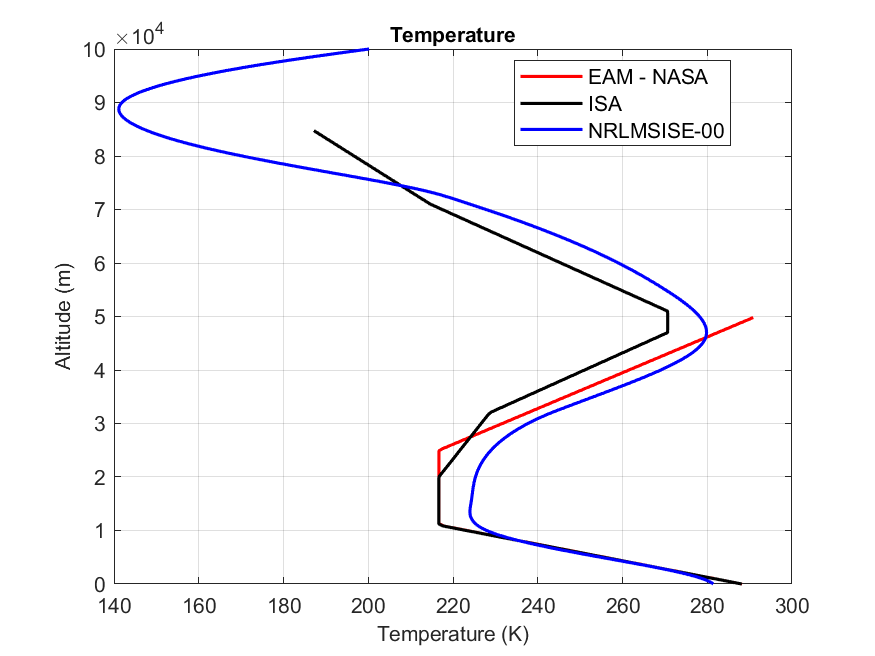
\includegraphics[width=\textwidth]{Figures/implementation/atmos/temperature_plot.png}
		\caption{Temperature Comparison}
		\label{fig:atmos_models_comp_temp}
	\end{minipage}
	\hfill
	\begin{minipage}{0.48\textwidth}
		\centering
		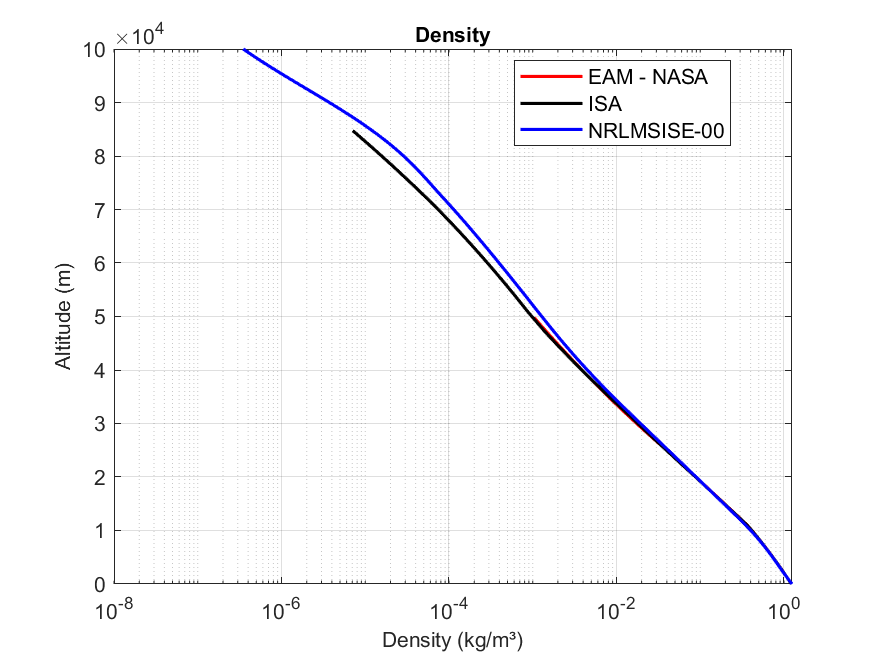
\includegraphics[width=\textwidth]{Figures/implementation/atmos/density_plot.png}
		\caption{Density Comparison}
		\label{fig:atmos_models_comp_density}
	\end{minipage}
\end{figure}

For the density profile, all the three models shwo a good agreement with minor a relative minor error between them. However, for the temperature profile, the analysis is not so straightforward. In the lower altitudes (up to 10 km), all models exhibit a roughly linear decrease in temperature, although NRLMSISE-00 shows slight irregularities. Between 10 and 20 km, \gls{isa} displays the characteristic plateau of the tropopause, while \gls{eam} and NRLMSISE-00 present smoother transitions. Above 20 km, significant differences become apparent: NRLMSISE-00 accurately captures the sharp temperature increase in the thermosphere, reflecting its detailed physical basis, whereas \gls{isa} maintains a simplified, smoothed profile, lacking this feature. \gls{eam} diverges from \gls{isa} but does not fully replicate the extreme rise observed in NRLMSISE-00. Overall, \gls{isa} serves as a practical but simplified model, NRLMSISE-00 provides higher accuracy at extreme altitudes, and \gls{eam} strikes a balance between simplicity and realism. This comparison underscores the distinct strengths and limitations of each model in representing atmospheric temperature variations.

Further anaylsis relevante to the atmospheric models performance is presented in table \ref{tab:atmos_model_speed}, Where the execution time of diferent number of functions calls are done. From this table, it is possible to understande that the NRLMISE00 model creates a huge impact when a simulation has a low descent ratio. This is because the NRLMISE00 model is more complex and computationally expensive than the other two.

\begin{table}[!htb]
    \centering
    \begin{tabular}{
    >{\columncolor[HTML]{FFFFFF}}l 
    >{\columncolor[HTML]{FFFFFF}}r
    >{\columncolor[HTML]{FFFFFF}}r
    >{\columncolor[HTML]{FFFFFF}}r }
    \hline
    {\color[HTML]{000000} No. Function Calls} & \multicolumn{1}{r}{\cellcolor[HTML]{FFFFFF}{\color[HTML]{000000} EAM \cite{noauthor_iso_nodate}}} & \multicolumn{1}{r}{\cellcolor[HTML]{FFFFFF}{\color[HTML]{000000} ISA \cite{noauthor_earth_nodate}}} & \multicolumn{1}{r}{\cellcolor[HTML]{FFFFFF}{\color[HTML]{000000} NRLMISES00 \cite{picone_nrlmsise00_2002}}} \\ \hline
    {\color[HTML]{000000} 1}                  & {\color[HTML]{000000} 0.8 \unit{\ms}}                                                                                           & {\color[HTML]{000000} 25.1 \unit{\ms}}                                                                                        & {\color[HTML]{000000} 46.6 \unit{\ms}}                                                                                                  \\
    {\color[HTML]{000000} 10}                 & {\color[HTML]{000000} 1.0 \unit{\ms}}                                                                                           & {\color[HTML]{000000} 5.1 \unit{\ms}}                                                                                           & {\color[HTML]{000000} 25.0 \unit{\ms}}                                                                                                 \\
    {\color[HTML]{000000} 100}                & {\color[HTML]{000000} 0.1 \unit{\ms}}                                                                                           & {\color[HTML]{000000} 19.1 \unit{\ms}}                                                                                          & {\color[HTML]{000000} 173.7 \unit{\ms}}                                                                                                \\
    {\color[HTML]{000000} 1000}               & {\color[HTML]{000000} 0.4 \unit{\ms}}                                                                                           & {\color[HTML]{000000} 173.9 \unit{\ms}}                                                                                         & {\color[HTML]{000000} 1.6 \unit{\s}}                                                                                                   \\
    {\color[HTML]{000000} 10000}              & {\color[HTML]{000000} 3.0 \unit{\ms}}                                                                                           & {\color[HTML]{000000} 1.3 \unit{\s}}                                                                                             & {\color[HTML]{000000} 21.0 \unit{\s}}                                                                                                  \\
    {\color[HTML]{000000} 100000}             & {\color[HTML]{000000} 28.1 \unit{\ms}}                                                                                          & {\color[HTML]{000000} 18.1 \unit{\s}}                                                                                           & {\color[HTML]{000000} 3.7 \unit{\minute}}                                                                                                 \\ \hline
    \end{tabular}
    \caption{Computational times for different number of function calls for the three atmospheric models.}
    \label{tab:atmos_model_speed}
\end{table} 

Taking into considerantion both profile and computational anaylis clearily theres some advantages of using all the models. \gls{eam} is quite accurate and fast for low altitudes, once \gls{isa} is in accordance to the others models for altitudes until 80 \unit{\km} and realtive fast, and finally the NRLMISE00 model is the slowest computationally but provides higher varitions in certain atmosphere regions. For the final implementation, the choice of the model considered in this work, \gls{isa} is the choosen model for all the analysis presented furter in this work, once it provides quite fast computational times and a wide range of altitudes, namely the range of the DAEDALUS \cite{riegler_daedalus_2018} project used in next section to validate the model.







